\documentclass{article}
\usepackage{arxiv}
\usepackage{multirow}
\usepackage[utf8]{inputenc} % allow utf-8 input
\usepackage[T1]{fontenc}    % use 8-bit T1 fonts
\usepackage{hyperref}       % hyperlinks
\usepackage{url}            % simple URL typesetting
\usepackage{booktabs}       % professional-quality tables
\usepackage{amsfonts}       % blackboard math symbols
\usepackage{nicefrac}       % compact symbols for 1/2, etc.
\usepackage{microtype}      % microtypography
\usepackage{lipsum}		    % Can be removed after putting your text content
\usepackage{graphicx}
\usepackage{amsmath}
\usepackage{arydshln}
\usepackage{booktabs}
\usepackage{natbib}
\usepackage{doi}
\usepackage{stackengine}
\usepackage{CJKutf8}
\usepackage{array}
\usepackage{xcolor}
\usepackage{marvosym}
\usepackage{natbib}
\setcitestyle{numbers,square}
% \usepackage[UTF8]{ctex}
\newcommand\xrowht[2][0]{\addstackgap[.5\dimexpr#2\relax]{\vphantom{#1}}}


\title{{\bf{ChineseWebText}}: Large-Scale High-quality Chinese Web Text Extracted with Effective Evaluation Model}

%\date{September 9, 1985}	% Here you can change the date presented in the paper title
\date{} 					% Or removing it

\author{
Jianghao Chen$^{1,2}$\thanks{Equal Contribution.} \quad
Pu Jian$^{1,2}$~\footnotemark[1] \quad
Tengxiao Xi$^{1,2}$~\footnotemark[1] \quad
Dongyi Yi$^{3}$~\footnotemark[1] \quad
Qianlong Du $^{1}$~\footnotemark[1] \quad \\
\bf{Chenglin Ding} $^{3}$ \quad
\bf{Guibo Zhu} $^{1,2,3}$\textsuperscript{\Letter}~ \quad
\bf{Chengqing Zong} $^{1,2}$ \quad
\bf{Jinqiao Wang} $^{1,2,3}$\quad
\bf{Jiajun Zhang} $^{1,2,3}$\textsuperscript{\Letter}~ \quad
\\
\small{$^1$ Institute of Automation, Chinese Academy of Sciences }\quad \\
\small{$^2$ School of Artificial Intelligence, University of Chinese Academy of Sciences }\\
\small{$^3$ Wuhan AI Research }\\
\texttt{\{chenjianghao2022,jianpu2023,xitengxiao2022\}@ia.ac.cn}\\
\texttt{\{qianlong.du,gbzhu,cqzong,jqwang,jjzhang\}@nlpr.ia.ac.cn}\\
}

% Uncomment to remove the date
%\date{}

% Uncomment to override  the `A preprint' in the header
%\renewcommand{\headeright}{Technical Report}
%\renewcommand{\undertitle}{Technical Report}
% \renewcommand{\shorttitle}{\textit{arXiv} Template}

%%% Add PDF metadata to help others organize their library
%%% Once the PDF is generated, you can check the metadata with
%%% $ pdfinfo template.pdf
% \hypersetup{
% pdftitle={A template for the arxiv style},
% pdfsubject={q-bio.NC, q-bio.QM},
% pdfauthor={David S.~Hippocampus, Elias D.~Striatum},
% pdfkeywords={First keyword, Second keyword, More},
% }

\begin{document}
\maketitle

\begin{abstract}

    During the development of large language models (LLMs), the scale and quality of the pre-training data play a crucial role in shaping LLMs' capabilities. To accelerate the research of LLMs, several large-scale datasets, such as C4 \cite{2020T5C4}, Pile \cite{2020_pile}, RefinedWeb \cite{2023refinedweb} and WanJuan \cite{2023wanjuan}, have been released to the public. However, most of the released corpus focus mainly on English, and there is still lack of complete tool-chain for extracting clean texts from web data. Furthermore, fine-grained information of the corpus, e.g. the quality of each text, is missing. To address these challenges, we propose in this paper a new complete tool-chain \textbf{EvalWeb} to extract Chinese clean texts from noisy web data. First, similar to previous work, manually crafted rules are employed to discard explicit noisy texts from the raw crawled web contents. Second, a well-designed evaluation model is leveraged to assess the remaining relatively clean data, and each text is assigned a specific quality score. Finally, we can easily utilize an appropriate threshold to select the high-quality pre-training data for Chinese. Using our proposed approach, we release the largest and latest large-scale high-quality Chinese web text \textbf{ChineseWebText}, which consists of 1.42 TB and each text is associated with a quality score, facilitating the LLM researchers to choose the data according to the desired quality thresholds. We also release a much cleaner subset of 600 GB Chinese data with the quality exceeding 90\%. The data, codes and the tool-chain are available in this website \footnote{\url{https://github.com/CASIA-LM/ChineseWebText}}.
    
    %High-quality and extensive pre-training data could enable the models to acquire a wide range of knowledge and abilities. While obtaining high-quality data, especially Chinese high-quality pre-training data, still have significant challenges, web data contains a vast array of diverse Chinese pretraining data plagued by a substantial amount of noise. In order to extract high-quality pre-training data from web for Chinese, in this paper we propose a new automatic pipline approach, \textbf{EvalWeb}. To ensure data quality, this approach first employs manually crafted rules to clean the raw crawled web data. Subsequently, a evaluaiton model is used to further process the cleaned data, thereby generating a quality score for each of them. Finally, we can use a appropriate threshold to filter out the high-quality pre-training data. With this approach, we process some crawled web data and release a 537 GB Chinese dataset \textbf{ChineseWebText1.0}, which is the largest public Chinese dataset. The results demonstrate that the accuracy of our cleaned data can exceed 95\%, which could effectively meet the requirements of pre-training. Notably, in the released dataset, we provide not only the final high-quality dataset but also intermediate data with quality scores, allowing users to re-filter the data according to their specific needs. Codes, data and models are available\footnote{\url{}}.
   
\end{abstract}

\section{Introduction}

Recent years have witnessed the rapid progress of large language models (LLMs). The models, such as GPT-3\cite{brown2020language}, BLOOM\cite{scao2022bloom}, LLaMA\cite{llama}, Falcon\cite{2023refinedweb}, PaLM\cite{chowdhery2022palm} and GPT-4\cite{GPT4}, become more and more powerful, even performing better than humans in some natural language understanding and generation tasks.  
During the development, it is evident that the scale and quality of pre-training data play a crucial role on LLM's capability. A large-scale and high-quality dataset is the foundation of LLMs and is the source of all the LLM's amazing capabilities.

%With the development of artificial intelligence, large language models (LLMs) garner significant attention and innovation in recent years. Models like GPT-3\cite{brown2020language}, GPT-4\cite{GPT4}, LLAMA\cite{llama}, OPT\cite{zhang2022opt} and some others \cite{chowdhery2022palm,nakano2022webgpt, touvron2023llama}, have provided substantial improvements in various applications, such as text generation, machine translation, question answering and dialogue. 
    

%The remarkable success of large language models can be primarily attributed to the extensive pool of pre-training data at their disposal. Pre-training data consists of vast text corpora compiled from diverse sources, and encompass billions of words and sentences across a wide range of domains and topics. Through training on these corpora, large language models develop a sophisticated understanding of language structures, grammatical rules, contextual relevance, and a substantial reservoir of knowledge. With pre-training data, LLM could learn a good capability of comprehending and generating natural language texts. As a result, the quality and quantity of pretraining data play a pivotal role in determining the knowledge and capability of large language models. 
 
In order to expedite the research on LLMs, several large-scale datasets have been made publicly available in recent years, such as C4 \cite{2020T5C4}, Pile \cite{2020_pile}, RefinedWeb \cite{2023refinedweb} and WanJuan \cite{2023wanjuan}. Previous studies usually collect the raw texts at first from various sources, such as Wikipedia, GitHub, ArXiv, Stack Exchange, and CommonCrawl, in which CommonCrawl data often accounts for the vast majority. Then, handcrafted rules are designed to filter out the raw data in three steps: extracting the data in the language of interested, filtering out the noisy texts with language-specific rules and data deduplication. It should be noted that, most of the previous studies mainly focus on the collection of English-centered texts, and there is lack of a complete tool-chain for extracting clean data centered in other languages, e.g. Chinese. Furthermore, previous work usually directly release the final data, without giving the fine-grained information of the text, such as the quality of each text, limiting the potential that assists LLM researchers to re-filter the data according to their desired quality threshold.

%After collecting a large number of raw data from web sources, such as ArXiv, GitHub, Wikipedia, Stack Exchange, CommonCrawl and so on, these work process them with well-designed extraction and filtering rules and then construct different types of large-scale datasets. However, most of these work are primarily focused on the collection of English texts, and there is a lack of a complete tool-chain for extracting Chinese clean data from web sources. Furthermore, these datasets only include the cleaned texts and overlook their corresponding refined information (e.g. the quality of each text), which could assist LLM researchers in re-filtering the texts according to their specific quality requirements.


%In order to train large language models, in recent years researchers\cite{touvron2023llama,gao2020pile,gunasekar2023textbooks,penedo2023refinedweb,scao2022bloom} usually construct pre-training data by mixing cleaned web data and curated high-quality datasets, such as arXiv, GitHub, Wikipedia, Stack Exchange, CommonCrawl and so on. In these work, \citeauthor{gao2020pile} (\citeyear{gao2020pile}) construct a 825GB English text dataset by combing 22 diverse and high-quality sub-datasets. Besides, by filtering and deduplicating web data from CommonCraw \citeauthor{penedo2023refinedweb} (\citeyear{penedo2023refinedweb}) build an English dataset RefinedWeb which includes 600 billion tokens. Different with them, \citeauthor{gunasekar2023textbooks} (\citeyear{gunasekar2023textbooks} build a code dataset with data from web and synthetically generated textbooks and exercises with GPT-3.5. However, these work mainly focus on the construction of English pre-training datasets, ignoring the importance of Chinese. Since each language possesses its unique characteristics, large language models trained on English data could not excel in comprehending and reasoning with Chinese text. Consequently, to enhance LLM's knowledge and capabilities for Chinese, this paper will mainly focus on the collection of Chinese pre-training data.

To address these problems, in this paper we introduce a new complete tool-chain \textbf{EvalWeb}, which could extract high-quality Chinese texts from raw web data. The whole process can be divided into two parts. The first part is similar to previous studies and mainly utilizes manually designed rules to filter out explicit noisy data, generating the initial Chinese clean data. This part processes the web texts with two modules: preparation module and processing module. The preparation module first employs a language identification model to extract Chinese data, and then adopts a hash-based deduplication algorithm to remove duplicate texts. The preprocessing module then handles the resulting data with well-designed rules, including length filtering, sensitive words filtering and filtering with Chinese character ratio. Previous studies usually stop after the usage of these rules. In contrast, we introduce the second part which is a quality evaluation module. Due to the diversity of web texts, the remaining dataset after the usage of filtering rules still contains a large number of low-quality text, which cannot be cleared using manually crafted rules. Consequently, we propose to design a BERT-based quality evaluation model for assessing all the remaining data, thereby generating a quality score for each text. Finally, we can select the high-quality Chinese data in the dataset according to the quality threshold. Using our complete tool-chain \textbf{EvalWeb}, we release the latest and largest Chinese dataset \textbf{ChineseWebText}, which consists of 1.42 TB data and each text is assigned a quality score, facilitating LLM researchers to select data according to a new quality threshold. We also release a much cleaner subset of 600 GB Chinese texts with quality exceeding 90\%.

%In this approach, we first use a preparation module to process the collected raw data from web. This preparation module first uses a language identification model to extract Chinese data from the fully web dataset, and then adopts a hash-based deduplication method to eliminate duplicate texts in the extracted data. In this way, we can obtain an initial Chinese web dataset. After that, a preprocessing module is employed to further process the texts in the initial Chinese web dataset. In this module we can filter out the explicit noises with some manually crafted rules, and then construct a filtered dataset. However, due to the diversity of web texts, the filtered dataset still has a large number of low-quality texts that cannot be cleared using manually crafted rules. Consequently, we propose to utilize a Bert-based evaluation model to assess all the filtered data, thereby generating a quality score for each text. Through this way, we can use a designed threshold to filter out all the high-quality data for Chinese. With this approach, we process 3.9 T source data from web, and construct a 672 GB Chinese dataset whose quality exceed 90\%. Furthermore, we also release a much larger Chinese dataset of 1.42 TB. In this dataset, each text is associated with a quality score, which allows LLM researchers to select data according to a new quality threshold. 


%we firstly adopt some manually crated filtering rules to remove explicit noises from web data, such as  pornography, violence, and advertising. In this stage, a language identification model will also be employed to filter out Chinese data from the fully web dataset, while a hash-based deduplication method will be used to eliminate duplicate texts. After that, a Bert-based evaluation model will be used to assess all the filtered data, thereby generating a quality score for each of the texts. Finally, we will design a appropriate threshold to filter out all the high-quality pre-training data for Chinese. With this approach, we process 3.9 T source data from web, and construct a 672 GB Chinese dataset whose quality exceed 90\%. Furthermore, we also release a much larger Chinese dataset of 1.42 TB. In this dataset, each text is associated with a quality score, which allows LLM researchers to select data according to a new quality threshold. 

%Recent researches \cite{gao2020pile,gunasekar2023textbooks,penedo2023refinedweb,scao2022bloom,shen2023slimpajamadc} have shown that filtered web data are very effective to train large language models. At the same time, there is a vast amount of Chinese text data available on the web. Consequently, this paper propose a new approach which could extract high-quality Chinese texts from web. In this approach, we first employ a set of manually crafted rules to conduct preliminary cleaning of the data gathered from web. Then we further use a BERT-based evaluation model to assess all the filtered data, thereby generating a quality score for each of them. Finally, by setting appropriate thresholds, we can filter out high-quality pre-training data from them. With this approach, in this paper we process 3.9T text data from web, and generate a 537 GB high-quality Chinese pre-training dataset which have been publicly released.  Notably, in the released dataset, we provide not only the final results but also intermediate data with quality scores, allowing users to re-filter the data according to their specific needs.
  
Our contributions can be summarized as follows:

(1) In this paper, we propose a new complete tool-chain \textbf{EvalWeb}, which could extract high-quality Chinese pre-training data from noisy web texts.

(2) In this paper, we release the latest and largest Chinese dataset consisting of 1.42 TB, and each text in this dataset is assigned a quality score according to our quality evaluation module. We further release a much cleaner subset of 600 GB Chinese texts with quality exceeding 90\%.

%a 672 GB Chinese dataset ChineseWebText, which is the largest and latest large-scale high-quality Chinese pre-training dataset.
%(3) In addition to the high-quality Chinese pre-training dataset ChineseWebText, we also release a much larger Chinese dataset of 1.42 TB, in which each text is associated with a quality score, allowing LLM researchers to select data according to their desired quality threshold.


\section{Related Work}

\textbf{Rule-based Text Filtering.} Rule-based text filtering methods are the dominant paradigm to identify content-rich and semantically coherent data from collected raw datasets with handcrafted rules. During the collection of pre-training data, there are a large number of text data on the web. However, these data include a lot of noise, such as violence, pornographic, advertisement and error characters. Consequently, in order to extract high-quality data, several rule-based methods have been proposed to explore how to automatically filter undesired content from noisy web data. In these work, deduplication\cite{lee_deduplicating_2022} methods are employed to remove duplicate text from the data, while some handcrafted rules \cite{raffel_exploring_2020,luccioni_whats_2021} are adopted to filter out violence, pornographic, advertisement and other explicit noisy data. Besides, perplexity \cite{wenzek_ccnet_2020} is also usually used to evaluate the fluency of the texts. However, these work mainly focus on English and lack a complete tool-chain for Chinese.

\textbf{Text Classification Model}. Different from rule-based text filtering methods, text classification model is an alternative approach to identify high-quality data with a well-designed classifier. The simplest text classification model is logistic regression\cite{brown2020language}, which uses the logistic function to calculate the probability values for each text, and then classifies them into positive or negative with a designed threshold. Currently, BERT\cite{devlin_bert_2018} and FastText\cite{joulin_bag_2017} are both commonly used text classification models. BERT is a transformer-based\cite{transformer} pre-training language model that has achieved remarkable performance in various text classification and understanding tasks. Through pre-training on masked language model and next sentence prediction tasks with a large dataset, this model learns powerful language understanding and representation abilities, which makes it perform well on text classification tasks. FastText\cite{joulin_bag_2017} is also a neural network based approach which is similar to CBOW\cite{word2vec}. It is characterized by its ability to train efficiently and quickly on large-scale data, while achieving competitive classification performance. In this paper, both of these two approaches will be employed to evaluate the qualities of the Chinese texts.  

\textbf{Datasets for Pre-training.} In recent years as the scale of pre-trained language models expands, there is a concomitant increase in the demand for large-scale pre-training datasets. Due to the convenience of acquisition and cost-efficiency associated with web-scraped data, it has progressively emerged as a pivotal source for pre-training datasets\cite{raffel2020exploring}. In these work, Gao et al. (2020) \cite{gao2020pile} build a 825 GB English corpus by mixing established natural language processing datasets and several newly introduced ones. This dataset covers 22 diverse high-quality subsets which derive from academic or professional sources, including PubMed Central, the FreeLaw Project, Stack Exchange, Books3\cite{presser2020books3}, OpenSubtitles\cite{tiedemann2016finding} and so on. Different from the work of Gao et al. (2020) \cite{gao2020pile}, Penedo et al. (2023)\cite{penedo2023refinedweb} demonstrate that properly filtered and deduplicated web data alone can also train a powerful model, even outperforming the LLMs trained on curated corpora. They use a pipeline approach to filter and deduplicate web data from CommonCrawl at very large scale and then release an English dataset which have 600 billion tokens. In addition, with data from web and synthetically generated textbooks and exercises with GPT-3.5, Gunasekar et al. (2023)\cite{gunasekar2023textbooks} build a code dataset which has 7B tokens. They mainly focus on the coding functions of LLMs, esecpically the writing Python functions. Moreover, He et al. (2023) \cite{he2023wanjuan} release a comprehensive multimodal dataset, which also contains texts in both Chinese and English, and is collected from a wide range of web sources. These public datasets mainly focus on English, and lack a complete tool-chain for extracting Chinese clean data from web sources. Furthermore, they only contain the cleaned texts, while missing the corresponding fine-grained information (e.g. the quality of each text) which could help LLM researchers to re-filter texts with new desired quality thresholds.


\section{Data Construction}

Due to the presence of substantial noise and irrelevant information on the web, extracting high-quality Chinese data from the web poses a significant challenge. In order to extract high-quality Chinese text from web effectively, in this paper we propose a pipeline system \textbf{EvalWeb}, which integrates mannual crafted rules and evaluation models. With this approach, we can effectively filter undesirable content such as offensive speech, advertisements and idle chatter, and then extract high-quality Chinese texts. As in Figure \ref{fig1}, it illustrates the overview of our proposed approach. For the crawled data from web, we first use a preparation module to process them, and then extract the monolingual Chinese data. After that, a preprocessing module will be used to further filter them with mannual crafted rules, including data length, sensitive words, proportion of Chinese characters and so on. Finally, a BERT-based evaluation model will be employed to assess the qualities of filtered data. By this way, we can generate a quality score for each of the text, and then use an appropriate threshold to extract the high-quality data as we required. Furthermore, 
considering computational cost and efficiency, we further propose to leverage knowledge distillation\cite{stanton2021does} techniques to train a FastText classifier, which can achieve similar performance with faster efficiency and lower computational costs.

\begin{figure}[htbp]
  \centering
  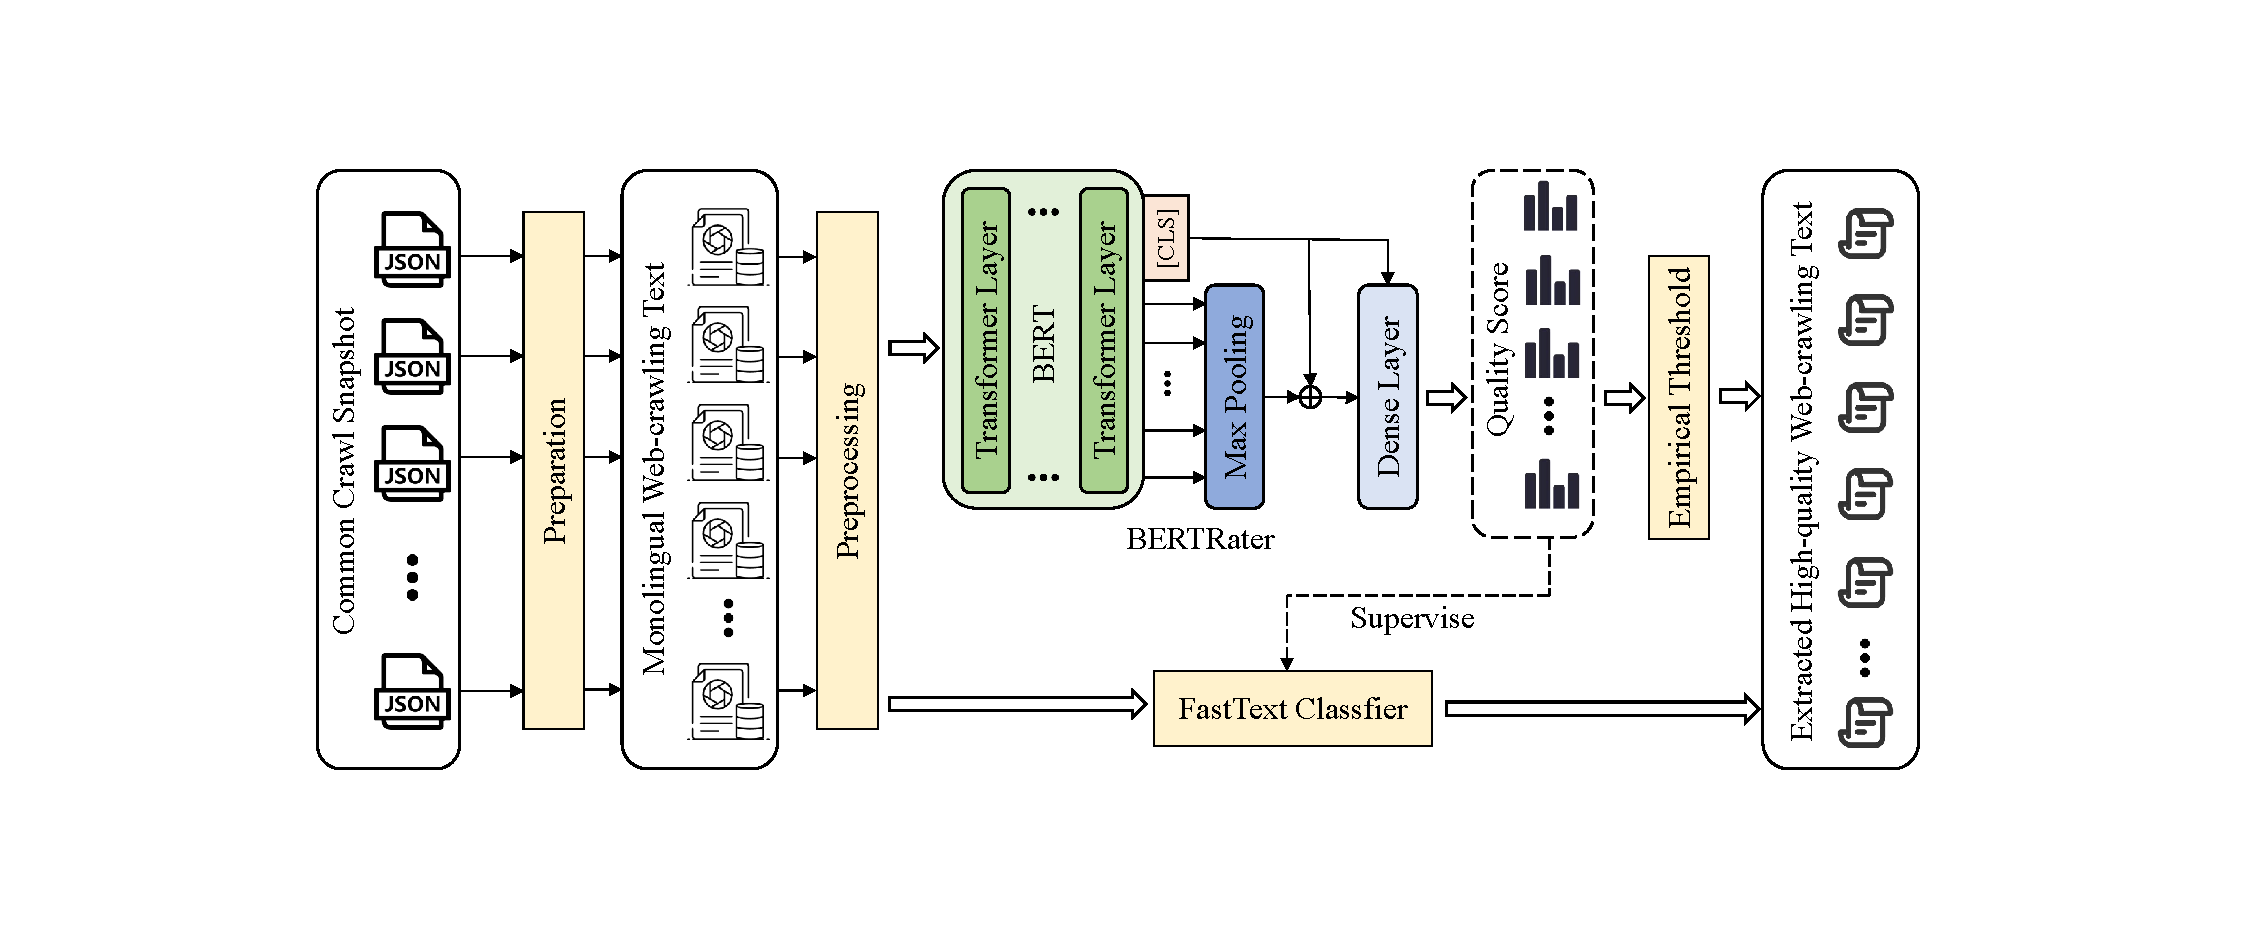
\includegraphics[width=1\textwidth]{picture/BERTRater_final.pdf}
  \caption{The architecture of our EvalWeb approach.}
  \label{fig1}
\end{figure}

\subsection{Data Collection and Preparation}

As a publicly accessible web scrape dataset, CommonCrawl has been running for 12 years and has accumulated petabytes of web data. Consequently, we regard it as the source of our web data. In this paper, we collect nine latest CommonCrawl snapshots from the internet, including "2021-43", "2022-05", "2022-21", "2022-27","2022-33","2022-49","2023-06","2023-14" and "2023-23". These obtained snapshots are compressed plain text, each of which is 8-10 TB in size (approximately 3 billion web pages). Each snapshot is regrouped into JSON format shards of 5 GB, where each item corresponds to a web page. 

Since the original CommonCrawl file is typically quite diverse and contains texts in many languages, to efficiently extract Chinese text data from it, we first employ a deduplication and language identification (LID) module to perform preliminary cleaning on the collected datasets. Following the work of CCNet\cite{wenzek_ccnet_2020}, in this module a Hash-based inter-string deduplication method is employed to remove duplicate text from different snapshots. Additionally, a well-trained language identification model\cite{grave2018learning}, which could support 157 languages, is applied to select Chinese data. By this way, we can obtain all the monolingual Chinese text data we required. 

\subsection{Preprocessing}

\begin{table}[htbp]
    \caption{ Examples for different filtering rules.}\label{Data Filtering Statistics}
    \centering
    \begin{tabular}{p{4cm} | p{9cm} }
    \toprule
     Filtering Operation & Example \\
     \midrule
     \multicolumn{1}{m{4cm}|}{Text Extraction}  & \multicolumn{1}{m{9cm}}{\begin{CJK}{UTF8}{gbsn} \{"url": "http://sarahokane.com/ywly/index.aspx",\newline "date\_download": "2022-05-28T10:17:39Z", \newline "length": 854, \newline "nlines": 17, \newline "source\_domain": "sarahokane.com", \newline "title": "合肥市建设投资控股(集团)有限公司", \newline \textcolor{red}{"raw\_content": " 乡村振兴和现代农业板块\textbackslash n乡村振兴与现代农业...注册资本4.39亿元。",} \newline ...\newline "language": "zh", \newline "bucket": "head"\} \end{CJK}}  \\
     \midrule
     \multicolumn{1}{m{4cm}|}{Length less than 200}  & \multicolumn{1}{m{9cm}}{\begin{CJK}{UTF8}{gbsn} "德国黑森州法兰克福AMazon数据中心" \end{CJK}}  \\
     \midrule
     \multicolumn{1}{m{4cm}|}{Average line length less than 10}  & \multicolumn{1}{m{9cm}}{\begin{CJK}{UTF8}{gbsn} "汽车资讯\textbackslash n汽车制造商\textbackslash n学车租车\textbackslash n俱乐部,汽车网,汽车报价,新车,汽车图片\textbackslash n汽车网,汽车报价,新能源,新车,汽车图片\textbackslash n南方网:汽车频道\textbackslash n维修,改装,车模,新车,用车\textbackslash n ......" \end{CJK}}  \\
     \midrule
     \multicolumn{1}{m{4cm}|}{Traditional Chinese characters}  & \multicolumn{1}{m{9cm}}{\begin{CJK}{UTF8}{bsmi} "有看過裝潢中的便利商店嗎?它可能內部還沒整備好,甚至根本是空盪盪的一片。但店門一定會上紅布條,寫著「XXX便利商店在此為您服務」。去過外縣市旅遊嗎?當你開著車要找某家店時,你大概不會開到正門口才看是不是你要找的店。" \end{CJK}}  \\
     \midrule
     \multicolumn{1}{m{4cm}|}{Proportion of Chinese characters fewer than 30\%}  & \multicolumn{1}{m{9cm}}{\begin{CJK}{UTF8}{gbsn} "线上买球平台\textbackslash u0006\textbackslash u0007、精准\textbackslash u0007\textbackslash u0005、可靠的传感技术解决方案及产品\textbackslash n\textbackslash nXSENS MTi 600系列 ...\textbackslash n\textbackslash n7 GNSS/INS\textbackslash n线上买球平台\textbackslash u0006,具有多个GN......</p>\textbackslash nMTi-G-710 GNSS/I...\textbackslash n<p><span style="font-size: 12px;">......" \end{CJK}}  \\
     \midrule
     \multicolumn{1}{m{4cm}|}{Occurrence of sensitive words more than 0.5 per line}  & \multicolumn{1}{m{9cm}}{\begin{CJK}{UTF8}{gbsn} "宝博体育强化创新引领,坚持“科技宝博体育”战略,构建“以企业为主体、市场为导向、产学研相结合”的科技创新体系。\textbackslash n2019年度大事记\textbackslash n友情链接:玩球直播nba 真钱滚球真人 金花三张牌赢钱 55直播nba 买球 手机轮盘app 亚博app在线登录 亚博app登录......" \end{CJK}}  \\
     \midrule
     \multicolumn{1}{m{4cm}|}{Internal duplication ratio greater than 50\%}  & \multicolumn{1}{m{9cm}}{\begin{CJK}{UTF8}{gbsn} "\textcolor{red}{“山东省民间融资机构宣传月活动”......活动期间吸引了当地市民\textbackslash{}n}2018年11月9日,\textcolor{red}{“山东省民间融资机构宣传月活动”......活动期间吸引了当地市民}的广泛关注,现场发放宣传资料600余份,解答市民疑问100余人次,德州广播电视台,德州日报,德州晚报全程采访报道。" \end{CJK}} \\
     \bottomrule
    \end{tabular}
\end{table}


After getting the monolingual Chinese web data, in this section we will focus on how to extract high-quality Chinese texts from them. Given the prevalence of violent, pornographic, advertising, and error characters in web data, we will first employ some manually crafted rules to filter out these noisy data. The details of these crafted rules are presented in the following.

 \textbf{Text Extraction} After the data preparation stage, there exists a substantial amount of redundant content, which holds little substantive value for subsequent analysis, such as irrelevant key-value pairs. To ensure the accuracy and efficiency of data analysis, we initially undertake the task of extracting all textual content from the entire dataset.

% \textbf{Traditional Chinese text \& Data Length} The goal of this paper is to construct a high-quality simplified Chinese dataset from web data. However, these data contain a large number of traditional Chinese characters. Therefore, we must clean these traditional Chinese texts firstly. During data processing, we will remove text data with more than 70\% of traditional Chinese characters. 

\textbf{Data Length} In web texts, a substantial portion of data consists of documents with short text lines which are separated by '\textbackslash n'. And the texts in different lines do not have significant semantic relevance to each other, which results in that these data are not useful for the training of language models. To eliminate excessively documents with short text lines, we will calculate the average text line length for each document and then remove documents with an average line length of fewer than 10 characters. Besides, during pre-training procedure, short text data usually contains limited information, making it ineffective in providing context and contextual information. Consequently, we will remove texts whose length is less than 200.

%Shorter data length typically indicates a lower information density. Given that the data is derived from web crawling, these short data entries often encompass non-essential content, such as advertisements. Therefore, we opt to filter out data entries where the average line length (separated by the '\textbackslash n' symbol) is fewer than 10 characters.

% \textbf{Perplexity} Utilizing a language model trained on Wikipedia, CCNet calculates and provides perplexity scores for each data entry. This perplexity metric can serve as a criterion to further filter and eliminate low-quality data. Data with a high perplexity score is more likely to contain ambiguous or contradictory information. Consequently, filtering out entries with elevated perplexity is a pivotal step in ensuring the accuracy and consistency of textual information. We remove data entries with a perplexity score greater than 4000.

% \textbf{Proportion of Characters} After analyzing some web data, we found that some data exhibit a notably low percentage of Chinese characters. And the rest of these data are filled with some other language characters, non-essential characters, special symbols, irrelevant markers, and so on. These data are unhelpful for the training of large language models. Consequently, we will remove the texts with fewer than 30\% Chinese characters.

\textbf{Proportion of Characters} The objective of this paper is to create a high-quality simplified Chinese dataset sourced from web data. Therefore, we firstly eliminate text data composed of traditional Chinese characters. Additionally, we found that some data exhibit a notably low percentage of Chinese characters. And the rest of these data are filled with some other language characters, non-essential characters, special symbols, irrelevant markers, and so on. These data are unhelpful for the training of large language models. Consequently, we will remove the texts with fewer than 30\% Chinese characters.

\textbf{Sensitive Words} In web data, there is a large amount of harmful texts, including sex, gambling, violence, discrimination, drugs, religion, and so on.  These texts can make large language models generate toxic contents, which have a big negative influence on society, nations and individuals. To avoid these issues, it is necessary to filter out harmful content from the web texts. Firstly, we collect a lot of harmful words and build a sensitive word list. After that, we count the sensitive words in each line of the texts. For one text, if the occurrence of sensitive words exceeds 0.5 per lines, we will regard it as a toxic text and will remove it from our dataset.

%Data from web scrapes, such as those obtained from Common Crawl, often contain sensitive terms or proprietary information. Without appropriate processing, this data can lead trained models to produce content in violation of legal standards, regulations, or national directives. To ensure the compliance of our training data and mitigate legal risks, we employ a filtering strategy based on a previously compiled list of sensitive terms, isolating data lines where the occurrence of such terms surpasses 0.5 per line (separated by the '\textbackslash n' symbol).

%Furthermore, considering our target audience predominantly uses Simplified Chinese, we also eliminate data entries where the proportion of Traditional Chinese characters exceeded 10\%, ensuring the research objectives are closely aligned with the readership's preferences.

\textbf{Internal duplication}
In the training of large language models, duplicate texts can significantly impact training efficiency and model performance. Although we have conducted deduplication in the first stage, subsequent analysis revealed that some duplicate information still exists in the texts. Therefore, we adopt a granularity of 13-gram for analysis, quantifying the proportion of repetitive 13-gram character sequences across all data. When the proportion of repeated 13-gram characters in a data sample exceeds 50\%, we opt to filter it out.

% Therefore, in this stage, we will perform deduplication on the texts once more. In this deduplication procedure, we will construct a list of 13-grams for each text, and then add it in to MinHash index. After that, Jaccard similarity will be used to determine whether a pair of texts should be regarded as a duplicate. The threshold of Jaccard similarity is setted to 0.5.    


%To rigorously examine this redundancy, we adopt a granularity of 13-gram for analysis, quantifying the proportion of repetitive 13-gram character sequences across all data. When the proportion of repeated 13-gram characters in a data sample exceeds 50\%, we opt to filter it out.

Through the aforementioned rigorous data preprocessing steps, a substantial amount of low-quality data is filtered out. After that, a quality evaluation model will be employed to evaluate the quality scores of the remaining data and then extract the high-quality data with a desired threshold. 

\subsection{Quality Evaluation}
\label{quality_evaluation}
\subsubsection{BERTEval}

In preprocessing procedure, we have used some handcrafted rules to remove the explicit noisy texts from our dataset. However, within the remaining data, there is still a considerable amount of low-quality text data, which cannot be filtered out with handcrafted rules. In order to extract the data of higher quality from them, in this section we further propose to design an evaluation model. In this approach, we will develop a BERT-based classification model to generate a quality score for each text, and then filter the high-quality data with a threshold. The details of the classification model are presented in the following.

%The preprocessing is able to remove some obviously explicit noisy through human crafted rules, such as line length, sensitive words, etc. However, content such as advertising or other unhelpful data for pre-training could not be removed. At the same time, we observed that most released datasets for pre-training often only contain the data itself without the author's evaluation of the data sample, especially the fine-grained evaluation of the quality (good or bad) of each data sapmle. Thus, we are motivated to design \textbf{BERTEval}, a text quality scoring model, to evaluate and score the data after preprocessing. The higher the score, the better the quality the model believes.


\textbf{Training Data Composition} While the evaluation in our current experiment targets CommonCrawl data, we believe the positive training samples should encompass a variety of text types, such as Wikipedia, e-books, poetry, news, and Q\&A data, to prevent the model from exhibiting bias toward deeming any specific text type as high quality. Since CommonCrawl data has a relatively high noise level overall, we directly sampled from CommonCrawl and used the sampling results as negative examples. Table \ref{bert_data} presents the detailed composition and quantity of the training data.
\begin{table}[htbp]
	\caption{Composition of BERTEval Training Data.}\label{bert_data}
	\centering
	\begin{tabular}{llc}
		\toprule
		Type     & Source     & Size ($\times 10^4 $) \\
		\midrule
		\multirow{8}{*}{Positive samples}   & Wikipedia & 12.50 \\ 
                                            & Sina News & 12.50 \\
                                    		& Cbooks & 12.50  \\
	                                        & Zhihu & 12.40 \\
	                                        & WikiQA & 0.90 \\
	                                        & Law & 0.40 \\
	                                        & Poetry & 0.20 \\
	                                        & GovReport & 0.13 \\
	    \midrule
            \xrowht[()]{10pt}
		Negative sample & CC-sampling & 55.00 \\
		\bottomrule
	\end{tabular}
\end{table}


\textbf{BERTEval Architecture} We utilized Tran-BERT-MS-ML-R\cite{wang_use_2022}, an effective AES model based on the BERT-base architecture, to evaluate the quality of the text obtained from web crawling. To reduce computational complexity, we opted to exclude the sub-document scale representation in Tran-BERT-MS-ML-R, which employs text segmentation at various scales as input. Instead, we focused solely on the text-scale representation, utilizing the $[CLS]$ embedding to extract pertinent information and structural features from the broadest perspective of the text. Simultaneously, the token-scale representation was derived from the sequence outputs of BERT. We anticipate that this token-scale representation will be instrumental in identifying and filtering out texts containing offensive language, sexually explicit terms, and frequent nonsensical vocabulary, typically absent in high-quality corpora. Let $x$ represent the text input. After the application of Max Pooling, the token-scale representation is concatenated with the text-scale representation and passed through a Dense Layer with Sigmoid activation, producing a text quality score $f(x|W)$ that falls within the $(0, 1)$ range.

% A well-performing, AES model of BERT-base architecture, Tran-BERT-MS-ML-R\cite{wang_use_2022}, is employed to score the quality of the web-crawled text. To minimize the computational complexity, we discard the sub-document scale representation in Tran-BERT-MS-ML-R that uses text segmentation at different scales as input. The text-scale representation is encoded by $[CLS]$ embedding for extracting information and structural features of text from the most global granularity. The token-scale representation is encoded by the sequence outputs of BERT. We anticipate that the token-scale representation will be beneficial in filtering texts containing offensive words, sexually explicit terms, and frequent nonsensical vocabulary. Such vocabulary is unlikely to appear in high-quality corpora. Take text input $x$, after Max Pooling, the token-scale representation is concatenated with text-scale representation and fed into a Dense Layer with Sigmoid activation to output a text quality score $f( x | W)$ that falls within the $(0, 1)$ range.

 


\textbf{Loss Function} In addition to the MSE loss\cite{mesgar_neural_2018}, we used the following two loss functions: Margin Ranking ($MR$) loss \cite{liu2021temp} and Cosine Similarity ($CS$) loss \cite{wang_use_2022}. Let $D$ denote the CommonCrawl corpus. Each negative sample $x_n$ is sampled from CommonCrawl associated with a fixed low score label $y_n$, which formed $D_n$. The positive sample, $x_p$, denotes curated corpora with ideal quality with a constant score $y_p$, which formed $D_p$. Throughout the training process, the labels for positive and negative samples are persistently $y_p$ and $y_n$, respectively. Moreover, it's noteworthy that a significant portion of high-quality texts is present within the CommonCrawl corpus. Given that the supervision employed is coarse-grained even somewhat inaccurate, it would be imprudent to solely rely on MSE loss to rigidly compel the model to fit these labels. For the $ML$ loss, losses only emerge when the ranking of quality scores for samples within each batch doesn't align with their respective labels. The $CS$ loss evaluates the correlation between quality scores and their supervision, rather than their absolute differences. Therefore, the combined loss is 
\begin{equation}
    \mathcal{L}(\boldsymbol{Y}, f(\boldsymbol{X }| W)) =\alpha MSE(\boldsymbol{Y}, f(\boldsymbol{X} | W))+\beta MR(\boldsymbol{Y}, f(\boldsymbol{X} | W))+ \gamma CS(\boldsymbol{Y}, f(\boldsymbol{X} | W)),
\end{equation}

where $\boldsymbol{Y}$ and $f(\boldsymbol{X} | W)$ are the quality score labels and predictions of a batch, respectively. Given the supervision is coarse-grained, we contend that the combined loss function offers valuable insights for enhancing our capability of BERTEval to assess the relative quality of texts. The BERTEval training process consists of the following two stages, which are shown in Fig 2.

\textbf{Pre-training Stage} At this stage, we extracted positive and negative samples at a 1:1 ratio from the CommonCrawl corpus and the curated corpora. We trained BERTEval based on the loss functions previously described. After this training stage, BERTEval acquired a preliminary ability to discern the quality of web-scraped texts, which will be elaborated in detail in the subsequent experiments section. 

\textbf{Self-training Stage} As mentioned before, there is a considerable proportion of texts with desired quality in the Common corpus $D_n$, which might introduce inaccurate supervision, resulting in neither increasing the epoch nor scaling up the training set leading to a detectable improvement in BERTEval. To ameliorate this problem, we adopt a self-training approach \cite{scudder1965probability}. Let $S_n$ denote a randomly sampled subset of $D_n$. In each self-training iteration, the parameters of BERTEval from the previous iteration, $W^t$, are used to generate the pseudo labels of $S_n$, and then BERTEval is retrained on sampled data in $S_n$ with pseudo labels to learn the new parameters $W^{t + 1}$\cite{mukherjee_uncertainty-aware_2020}. It's worth noting that since the positive samples originate from large-scale, high-reliability, curated corpora that do not require pseudo-labeling, we exclusively sample instances with pseudo-labels being $y_n$. The self-training stage can be formulated as:
\begin{equation}
W^{t+1} = \mathop{\arg\min} \limits_{W} \mathbb{E}_{\boldsymbol{X}_p^l \subset D_p} \mathbb{E}_{S_n \subset D_n} \mathbb{E}_{\boldsymbol{X}_n^l \sim p(x_n| W^{t}), \boldsymbol{X}_n^l \subset S_n}\{\mathcal{L}(\boldsymbol{Y}_p^l \oplus \boldsymbol{Y}_n^l, f(\boldsymbol{X}_p^l \oplus \boldsymbol{X}_n^l | W))\}.
\end{equation}
where $\boldsymbol{X}_p^l$ and $\boldsymbol{X}_n^l$ denote the vectors consisting of $l$ randomly sampled samples from $D_n$ and $S_n$, respectively, and $\boldsymbol{Y}_p^l$ and $\boldsymbol{Y}_n^l$ are the corresponding constant vector labels. Since the output layer is activated by Sigmoid, the quality score $f(x | W)$ can also be regarded as a probability of positive samples $p(y_p | x; W)$. Based on the idea of preferring pseudo-labels with high confidence, in iteration $t$, the probability of selecting each sample $x_n \in S_n$ is denoted by 
\begin{equation}
p(x_n|W^t) = \frac{p(y_n|x_n; W)}{\sum_{x \in S_n} p(y_n|x; W)},
\end{equation}
which is the normalization of $p(y_n|x_n; W)$. Heuristically, we avoid sampling the web-crawled texts where $p(y_n|x_n; W)$ falls within the last $K$ proportions. The value of $K$ is informed by our sampling observations from the CommonCrawl dataset. 

%%Given that BERTEval has already produced high-confidence predictions for certain samples, the gains from self-training would be minimal if we only select those with the highest confidence pseudo-labels. Thus we did not solely opt for the top $l$ samples based solely on their pseudo-label confidence.

\subsubsection{FastText-based Evaluation Model}

\begin{table}[htbp]
	\caption{Composition of FastText Training Data.}\label{fasttext_data}
	\centering
	\begin{tabular}{llc}
		\toprule
		Type     & Source     & Size ($\times 10^4 $) \\
		\midrule
		\multirow{8}{*}{Positive samples}   & Baike & 20 \\ 
                                            & Cbook & 20 \\
                                    		& Zhidao& 20  \\
		                                    & China News & 20 \\
	                                        & Zhihu & 20 \\
	                                        & WikiQA & 10 \\
	                                        & other news & 10 \\
	                                        & BERT-positive & 40 \\
	    \midrule
            \xrowht[()]{10pt}
		Negative sample & BERT-negative & 160 \\
		\bottomrule
	\end{tabular}
\end{table}

To further enhance data processing efficiency and reduce hardware resource requirements, in this paper we also develop a text evaluation model based on FastText\footnote{https://github.com/facebookresearch/fastText} in addition to BERTEval. FastText is libiary for efficient learning of word representations and text classificaiton. Compared to other classification models, such as SVM, logistic regression, and BERT, FastText could significantly reduce training and inference time while maintaining classification performance. 

In the last section, we have built a BERT-based evaluation model BERTEval which performs a good performance on the quality evaluation of Chinese texts. With this model, we can classify the preprocessed web data into high-quality texts (positive) and low-quality texts (negative). Inspired by the idea of knowledge distillation, we will use these classified texts to guide the training of our FastText model. In our approach, we select 400,000 high-quality texts classified by BERTEval as our positive data, while choosing 1,600,000 low-quality texts as our negative data. In order to increase the diversity of training data, our positive data also include some high-quality Chinese data from some other websites and books, such as Baidubaike, Zhihu, Cbook, ChinaNews and so on. These data have been manually proofread and processed. In this way, we can build a good training dataset with 3200K samples. As shown in Table \ref{fasttext_data}, it presents the composition of our training data.

After collecting these training data, we will use a word segmentation tool to process all the texts, and then input the processed data into FastText to train the model. Through this approach, we can obtain a more efficient quality evaluation model.

%During training procedure, the quality of training data has a big influence on the performance of evaluation models. As shown in Table \ref{fasttext_data}, it presents the composition of our training data. In this dataset, the positive data are mainly from two sources: (1) High-quality Chinese data collected from different websites and books, such as Baidubaike, Zhihu, Cbook, ChinaNews and so on. These data have been manually proofread and processed. (2) The CommonCrawl data with high quality scores which are evaluated by BERTEval. 
%At the same time, we collect the texts with 


%\textbf{Tarining Data Composition} For FastText, the positive samples come from two categories. One part of data is obtained from mainstream Chinese websites through web crawling, such as baike, zhidao, zhihu, etc. These data have been carefully processed and cleaned to ensure their high quality. Another part is consist of positive examples that have been prepossessed and classified by BERTEval. The combination of these two types of data forms the positive training examples for FastText. There is a total of 1.6 million positive examples. The negative samples, consist of 1.6 million samples, are drawn from the text with low quality scores by BERTEval. The composition of training data is presented in Table \ref{fasttext_data}.



%While the inference speed of BERTEval is acceptable (relative to LLM pre-training), we desire a scoring model of high accuracy with lower time consumption. Thus we propose a knowledge distillation-like method\cite{sun2019patient}, with BERTEval serving as the teacher model, to train a FastText\cite{joulin_bag_2017} classifier. FastText balances performance and computational complexity by sacrificing a certain degree of accuracy in exchange for faster and more efficient processing.

%\textbf{Tarining Data Composition} For FastText, the positive samples come from two categories. One part of data is obtained from mainstream Chinese websites through web crawling, such as baike, zhidao, zhihu, etc. These data have been carefully processed and cleaned to ensure their high quality. Another part is consist of positive examples that have been prepossessed and classified by BERTEval. The combination of these two types of data forms the positive training examples for FastText. There is a total of 1.6 million positive examples. The negative samples, consist of 1.6 million samples, are drawn from the text with low quality scores by BERTEval. The composition of training data is presented in Table \ref{fasttext_data}.


%\textbf{Knowledge Distillation and Training} The objective of knowledge distillation is to improve the performance of the student model ( FastText ) by leveraging the knowledge learned by the teacher model ( BERTEval ). Since the training data has been classified by BERTEval or processed manually, incorporating BERTEval's prior knowledge, this training process can be seen as a distillation process. Subsequent experimental results proved that the training method could effectively improve FastText's classification results. With relatively small training time, FastText achieves competitive results with BERTEval.


 \subsubsection{Evaluation Model Comparison}
 
 In order to compare the performance of different evaluation models, in this section we evaluate them on a test set which includes 300 samples. Here we first list other two baseline quality evaluation models: regression-based approach and perplexity-based approach.
 
 \textbf{Regression-based Evaluator}
 
 Following the work of Gururangan et al. (2022) \cite{gururangan_whose_2022}, we combine logistic regression with a word frequency-based vertorizaiton method to conduct text classification on the testset. In this approach, logistic regression is used to calculate a probability value for each sample, and then a threshold is adopted to determine whether the data point should be classified into positive or negative. 
 

 %we employ a word frequency-based vectorization method in combination with logistic regression for text classification of the data. Logistic regression models the probability of data belonging to the positive class. We use logistic regression to calculate the evaluation probabilities for each sample. Then, we use these probabilities to determine whether each data point should be classified as positive or negative.
 
 \textbf{Perplexity-based Evaluator}
 
 Perplexity could effectively measure the difficulty of a language model in predicting tokens and reflect the fluency of the input texts. Following the work of Wenzek et al. (2020) \cite{wenzek_ccnet_2020}, we utilize a well-trained language model to calculate the perplexity of the texts and classify them with a threshold based on perplexity values. The samples with lower perplexity values will be classified into positive.
 
 \textbf{Comparison Results}
 
 During testing procedure, we will classify the samples of testset with Regression, Perplexity, BERTEval and FastText models repectively, and then compute the precisions of them on positive data. As in Table \ref{results}, it shows the precisions of different evaluaiton models on the testset. TP represents the number of "True Positive" samples, while FP represents the number of "False Positive" samples. From this table, we can see that our BERTEval evaluaiton model gets a much better performance than the regression and perplexity approaches. Besides, benefiting from the good classified results of our BERTEval model, the FastText-based model could further improve the classification precision. This result indicates that using BERTEval to guide the construction of the FastText-based evaluation model is effective. And with this FastText-based evaluation model, our EvalWeb tool-chain could achieve a better performance while effectively improving processing efficiency and resource utilization.

%We calculated the proportion of positive examples classified by each model that accurately meets all four perspectives. A key point is that the objective of data classification is to improve the quality of data. And samples classified as positive will be used for further pre-training purposes. Therefore, we mainly focused on evaluating the precision, which indicates the proportion of truly positive samples. The results are presented in Table \ref{results}.The results indicate that both of our proposed methods, FastText, BERTEval, have shown impressive performance compared to Regression and Perplexity. Moreover, benefiting from the effect of data distillation, FastText's precision even surpassed BERTEval. 

% %\begin{table}[htbp]
% %	\caption{Classification Results }\label{results}
% % 	\centering
% % 	\begin{tabular}{lccc}
% % 		\toprule
% % 		Model      & Recall(\%) & F1(\%)  \\
% % 		\midrule\xrowht[()]{10pt}
% % 		Origin & 53 &  & \\ 
% % 		\xrowht[()]{10pt}
% % 		Regression & 49.57 & 72.96 & 59.03  \\
% % 		\xrowht[()]{10pt}
% % 		PPL &   &   &  \\
% % 		 \xrowht[()]{10pt}
% %         FastText&    &  & \\
% % 		\xrowht[()]{10pt}
% %         BERTEval & 73.79 & 47.80 & 58.02 \\	  
% % 		\bottomrule
% % 	\end{tabular}
% % \end{table}

 \begin{table}[htbp]
 	\caption{Classification results of different evaluation models.}\label{results}
 	\centering
 	\begin{tabular}{lccc}
 		\toprule
 		Model      & Precision(\%) & TP+FP & TP \\
 		\midrule\xrowht[()]{10pt}
 		Regression & 49.57 & 234 & 116 \\
 		\xrowht[()]{10pt}
 		Perplexity &  63.27 & 245 & 155 \\
 		 \xrowht[()]{10pt}
          BERTEval & 73.79 & 103 & 76\\
 		\xrowht[()]{10pt}
        FastText&  \textbf{81.58} & 76 & 62 \\	  
 		\bottomrule
 	\end{tabular}
 \end{table}


\subsection{Quality Control}\label{quality_control}

 \begin{figure}[htbp]
  \centering
  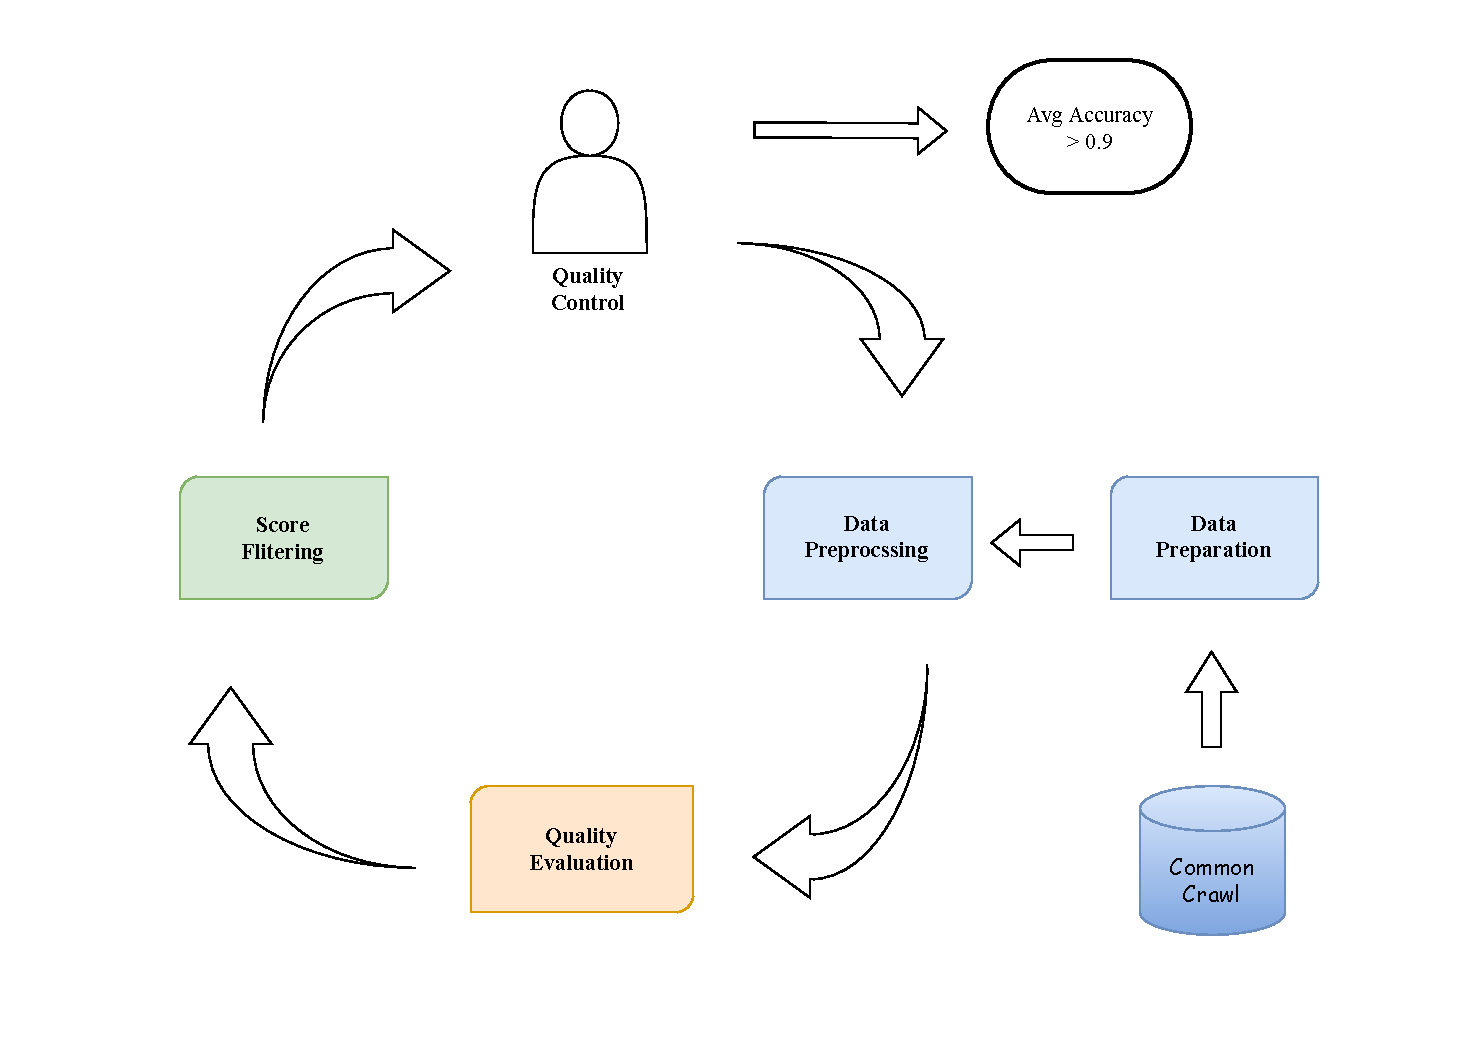
\includegraphics[width=0.9\textwidth]{picture/human_quality_control_final.pdf}
  \caption{Quality Control.}
  \label{fig2}
 \end{figure}

In section 3.3, after filtering data with a desired quality threshold, we can obtain a Chinese text dataset. In order to ensure the quality of this dataset, We will hire some human evaluators to evaluate its quality. In this method, we will randomly sample 1000 examples from the dataset for three times. After that, three human evaluators will be hired to assess the quality of these data respectively, and the quality of these data is required to be evaluated from the following four aspects: 

%To validate the effectiveness of the data quality evaluation, we conducted huamn sampling from evaluation results to ensure the scores given by the model accurately reflect the quality of the data. Specifically,after preprocessing and quality evaluation, we perform three rounds of sampling from the data scoring by qulity evaluation model. Each round involved randomly selecting 1000 data samples and applying the scoring model to assign scores to them. Then, we conducted huamn evaluations to assess the quality of this round data from various perspectives. The evaluators are instructed to consider the following aspects during the evaluation: 

\begin{itemize}
\item \textbf{Informativeness}: Whether the text contains enough knowledge and information,  or is just meaningless crap.
\item \textbf{Fluency}: Whether the text has formatting issues, capitalization mistakes, or evident grammatical errors that impair readability.
\item \textbf{Coherence}: Whether the text progressively forms a coherent body of information on a topic through its successive sentences. 
\item \textbf{Toxicity}: Texts used for pre-training should endeavor to exclude offensive remarks, sexually explicit content, and politically sensitive statements to mitigate potential generative risks.
 \end{itemize}
 
 
 \begin{table}[htbp]
    \caption{Data samples in json format. The higher score of Sample 1 versus the lower score of Sample 2 demonstrates their differing text qualities, with Sample 1 having better quality than Sample 2. }
    \label{Data Example Format}
    \centering
    \begin{tabular}{p{2.5cm} p{12cm} }
    \toprule
      \textbf{Key} & \textbf{Value}\\
     \midrule
        <\textbf{title}> &\begin{CJK}{UTF8}{gbsn}"潍坊银行2021年上半年净利润同比增长29.57\% 不良率降至1.10\%\_财经\_中国网"\end{CJK}\\
        <\textbf{score}>& 0.95 \\
        <\textbf{text}> & \multicolumn{1}{m{12cm}}{\begin{CJK}{UTF8}{gbsn} "潍坊银行2021年上半年净利润同比增长29.57\% 不良率降至1.10\%\textbackslash n中国网财经8月24日讯 潍坊银行昨日披露2021年二季度信息报告显示,截至2021年6月末,潍坊银行资产总额1920.44亿元,较上年末增长9.34\%;负债总额1789.16亿元,较上年末增长10.54\%。2021年上半年,潍坊银行实现净利润6.09亿元,同比增长29.57\%。\textbackslash n资产质量方面,截至2021年6月末,潍坊银行不良贷款率1.10\%,较上年末下降0.13个百分点。\textbackslash n资本金方面,截至2021年6月末,潍坊银行资本充足率、核心一级资本充足率、一级资本充足率分别为11.66\%、7.89\%、10.13\%,分别较上年末下降1.89、0.89、1.15个百分点。" \end{CJK}}  \\
        <\textbf{url}> & \url{http://finance.china.com.cn/news/special/2021bnb/20210824/5638343.shtml}\\
        <\textbf{source\_domain}> & \url{finance.china.com.cn}\\
         \midrule
        <\textbf{title}> &\begin{CJK}{UTF8}{gbsn}"上海巨也仪器设备有限公司"\end{CJK}\\
        <\textbf{score}>& 0.19 \\
        <\textbf{text}> & \multicolumn{1}{m{12cm}}{\begin{CJK}{UTF8}{gbsn} "石子冲击试验仪\textbackslash n现货提供石子冲击试验机\textbackslash n现货提供石子冲击试验机符合SAE、ASTM、VDA、GM、Ford、Mazda、JIS、Nissan、及Toyota等的测试要求。石子冲击试验机(欢迎实地考察)满足:大众、神龙、通用、日产、马自达、丰田、本田、福特等汽车厂家试验。\textbackslash nNS耐石子冲击性能试验机\textbackslash n耐石子冲击性能试验机主要用于、德系日系、美系汽车厂家试验方法,它能准确再现由飞溅的砂砾造成的破化现象, 适用于外涂层粘聚性破坏试验、涂层系统中不同层间粘合性破坏试验、抗剥落的*涂膜厚度、塑料及玻璃的抗剥落、抗碰撞、抗磨损测试等相关试验。\textbackslash n石子冲击试验机(欢迎实地考察)\textbackslash n石子冲击试验机(欢迎实地考察)符合SAE、ASTM、VDA、GM、Ford、Mazda、JIS、Nissan、及Toyota等的测试要求。满足:大众、神龙、通用、日产、马自达、丰田、本田、福特等汽车厂家试验。\textbackslash n漆膜抗石击试验仪\textbackslash n漆膜抗石击试验仪符合SAE、ASTM、VDA、GM、Ford、Mazda、JIS、Nissan、及Toyota等的测试要求。\textbackslash n石子冲击试验机/抗石子冲击仪\textbackslash n巨也仪器!有大量现货提供,欢迎客户随时来厂参观与指导!" \end{CJK}}  \\
        <\textbf{url}> & \url{http://www.juyesh.com/SonList-1094890.html}\\
        <\textbf{source\_domain}> & \url{www.juyesh.com}\\
        \bottomrule
    \end{tabular}
\end{table} 
 
 
 During evaluation procedure, each text is assigned a label of either "True" or "False." "True" indicates that the data meets the quality requirement of pre-training in all four aspects, while "False" signifies that the text is noisy to some extent. After completing all the evaluations, we will calculate the average accuracy of these three evaluators. If the average accuracy could exceed 0.9, the filtered Chinese dataset is considered to be a high-quality dataset. Otherwise, we believe that there is still some noisy text in the dataset, and we need to optimize the preprocessing and evaluation modules again, and reprocess the dataset until it meets the quality requirements. The architecture of quality control process is illustrated in Figure \ref{fig2}. 
 
 
 %To facilitate the evaluation process, we requested the evaluators to assess each data instance based on these four aspects and assign a binary label (0 or 1) indicating whether the data is suitable for the pre-training phase. For scoring models, we consider samples with a score above 0.8 as suitable for pre-training. Based on the manual labels, we calculated the precision of the three sampling rounds. We consider the model training to be satisfactory if the average precision of the three sampling rounds exceeds 70\%. If this criterion is not met, we will re-adjust the parameter settings in the preprocessing stage, such as the minimum length, duplication ratio, and character analysis method, as well as the settings in the training stage, such as the training data distribution ratio. The entire process is illustrated in Figure \ref{fig2}.
 

%     %   \multirow{5}{*}{Sample 3}
%     %     &title &\begin{CJK}{UTF8}{gbsn}"邹平金钰磨料有限公司"\end{CJK}\\
%     %     &url & \url{http://www.jy-abrasive.com/NewsDetail/2413642.html}\\
%     %     &source domain & \url{www.jy-abrasive.com}\\
%     %     &score& 0.590 \\
%     %     &text & \multicolumn{1}{m{13cm}}{\begin{CJK}{UTF8}{gbsn} "喷丸喷砂工艺的应用\textbackslash n喷丸喷沙主要用于钢铁等金属制品的表面处理\textbackslash n1.工件涂镀、工件粘接前处理喷砂能把工件表面的锈皮等一切污物清除,并在工件表面建立起十分重要的基础图式(即通常所谓的毛面),而且可以通过调换不同粒度的磨料,达到不同程度的粗糙度,大大提高工件与涂料、镀料的结合力。或使粘接件粘接更牢固,质量更好。\textbackslash n2.铸锻件毛面、热处理后工件的清理与抛光喷砂能清理铸锻件、热处理后工件表面的一切污物(如氧化皮、油污等残留物),并将工件表面抛光提高工件的光洁度,能使工件露出均匀一致的金属本色,使工件外表更美观,达到美化装饰的作用。\textbackslash n3.机加工件毛刺清理与表面美化喷砂能清理工件表面的微小毛刺,并使工件表面更加平整,消除了毛刺的危害,提高了工件的档次。并且喷砂能在工件表面交界处打出很小的圆角,使工件显得更加美观、更加精密。\textbackslash n4.改善零件的机械性能机械零件经喷砂后,能在零件表面产生均匀细微的凹凸面(基础图式),使润滑油得到存储,从而使润滑条件改善,并减少噪声提高机械使用寿命。\textbackslash n5.光饰作用对于某些特殊用途工件,喷砂可随意实现不同的反光或亚光。" \end{CJK}}  \\
%     % \midrule   
%         <\textbf{url}> & \url{http://www.gh-esports.com/news/shownews.php?lang=cn&id=218}\\
%         <\textbf{source\_domain}> & \url{www.gh-esports.com}\\
%      \midrule
%         <\textbf{title}> &\begin{CJK}{UTF8}{gbsn}"比了购"\end{CJK}\\
%         <\textbf{score}>& 0.035 \\
%         <\textbf{text}> & \multicolumn{1}{m{12cm}}{\begin{CJK}{UTF8}{gbsn}  "北极狐kanken背包怎么样\textbackslash n丽贝乐自营旗舰店\textbackslash n保而防护腰怎么样\textbackslash n蹀愫女鞋质量怎么样\textbackslash n麦拉贝拉纱布口水巾好吗\textbackslash nlacoste网上专卖店\textbackslash n雅戈尔羊毛衫怎么样\textbackslash n鲨鱼是bape还是aape\textbackslash ntakami在哪里可以买到\textbackslash n化氏专卖店实体店\textbackslash n雪花秀滋盈适合夏天吗\textbackslash n雪花秀的面霜好用吗\textbackslash n后化妆品和雪花秀哪个好用吗\textbackslash n雪花秀气垫哪款比较好\textbackslash n雷朋眼镜到底是玻璃的还是树脂的\textbackslash n佑天兰油痘皮适合吗\textbackslash n德国芭乐雅眼霜好不好\textbackslash n花王和尤妮佳的区别\textbackslash n尤妮佳的尿不湿厚度怎么样\textbackslash n美赞臣和惠氏启赋对比\textbackslash n启赋和金领冠哪个好\textbackslash n26\textbackslash n快40用娇兰帝皇蜂姿还是御庭兰花\textbackslash n娇兰瞬间浓香水礼盒怎么样\textbackslash n宜宾哪个商场娇兰专柜\textbackslash n娇兰m375跟哪个像\textbackslash n亲润cc霜效果怎么样\textbackslash n娇韵诗和亲润哪个好用\textbackslash n亲润豆乳哪里有卖3z\textbackslash n海威特i31跟i39哪个好\textbackslash n海威特m8和m13哪个好\textbackslash n南昌有安德玛专卖店吗\textbackslash n黛尔佳人的东西好吗\textbackslash n可可丽人专柜怎么样\textbackslash n俏卡莲口红好不好试色\textbackslash n贝比玛玛米饼会上火吗\textbackslash n欧珀莱柔润洁面膏怎么样\textbackslash ncrocs网店网址折扣店\textbackslash ncrocs洞洞鞋好在哪\textbackslash n颐莲祛斑霜有效果吗\textbackslash n小猪班纳旗舰店母婴\textbackslash n倍量深圳专卖店\textbackslash n夏娃之秀魔力挺效果好不好\n三雄极光的灯好不好" \end{CJK}}  \\
%         <\textbf{url}> & \url{http://www.cbeeta.org.cn/cueecbvy2/}\\
%         <\textbf{source\_domain}> & \url{www.cbeeta.org.cn}\\
    %  \midrule 
 
\begin{table}[htbp]
    \caption{Overview of output datasets.}
    \label{total_remain_size}
    \centering
    \begin{tabular}{cp{2cm}p{2cm}p{2cm}}
    \toprule
    \multirow{3.5}{*}{Snapshot}   & \multicolumn{3}{c}{Data Size(GB)} \\
                                \cmidrule{2-4}
                                & \centering Monolingual Chinese Data & \centering ChineseWebText Dataset & \centering Cleaner Subset \arraybackslash \\
    \midrule 
    \xrowht[()]{5pt}
    \textbf{2021-43} & \centering 505.92 & \centering 187.57 & \centering 78.95 \arraybackslash\\
     \xrowht[()]{5pt}
    \textbf{2022-05} & \centering 442.47 & \centering 164.96 & \centering 69.44 \arraybackslash\\
     \xrowht[()]{5pt}
    \textbf{2022-21} & \centering 443.57 & \centering 166.75 & \centering 70.19 \arraybackslash\\
     \xrowht[()]{5pt}
    \textbf{2022-27} & \centering 417.95 & \centering 149.41 & \centering 62.70 \arraybackslash\\
     \xrowht[()]{5pt}
    \textbf{2022-33} & \centering 369.56 & \centering 123.70 & \centering 51.98 \arraybackslash\\
     \xrowht[()]{5pt}
    \textbf{2022-49} & \centering 445.29 & \centering 160.87 & \centering 67.76 \arraybackslash\\
     \xrowht[()]{5pt}
    \textbf{2023-06} & \centering 396.40 & \centering 173.47 & \centering 74.19 \arraybackslash\\
     \xrowht[()]{5pt}
    \textbf{2023-14} & \centering 441.46 & \centering 150.04 & \centering 63.33 \arraybackslash\\
     \xrowht[()]{5pt}
    \textbf{2023-23} & \centering 371.96 & \centering 143.93 & \centering 61.28 \arraybackslash\\
    \midrule\xrowht[()]{5pt}
    \textbf{Total} & \centering 3834.58 & \centering 1420.70 & \centering 599.82 \arraybackslash\\
    % \midrule
    \bottomrule
    \end{tabular}
\end{table}
 
 \begin{table*}[htb]
\centering
    %\small
     \caption{ The comparison of different pre-training datasets.}
    \label{Dataset Compare}
    \begin{tabular}{ccccc}
    \toprule
    \textbf{Dataset} & \textbf{Lang.} &\textbf{Availability}& \textbf{Pubilc Size} & \textbf{Scoring} \\
    \midrule
    C4\cite{2020T5C4}   & EN & Public &  807GB  & NO   \\  
    The Pile\cite{2020_pile} & EN & Public & 825GB  &   NO \\ 
    REFINEDWEB\cite{2023refinedweb} & EN & Public& 2.8TB    &  NO  \\
    WuDaoCorpora\cite{2021WuDaoCorpora}  & ZH & Pratly Public & 200GB  &  NO \\
    ROOTS-zh\cite{2023roots} & ZH & Public &  265GB   &  NO\\
    WanJuan1.0-zh\cite{2023wanjuan}   & ZH & Public & 550GB  & NO\\
    \textbf{ChineseWebText} (Ours)        & ZH & Public & 1.4 TB &  YES \\
    \textbf{Cleaner Subset} (Ours)        & ZH & Public & 600 GB &  YES \\
    \bottomrule
    \end{tabular}
   
\end{table*}
 
 
\subsection{Dataset Statistics and Comparison}\label{dataset_statistics_comparison}


After processing the collected CommonCrawl data with preprocessing and quality evaluation modules, this paper constructs a clean Chinese dataset ChineseWebText, which consists of 1.42 TB data. As shown in Table \ref{Data Example Format}, each text in this dataset is assigned a quality score which is generated by the quality evaluation model BERTEval. In this table, a larger quality score signifies a higher text quality. With these quality scores, LLM researchers could further select data according to a desired quality threshold. In addition to ChineseWebText, this paper also release a much cleaner subset of nearly 600 GB Chinese texts, which is built by choosing data from ChineseWebText with quality scores in the top 40\%. Through manual evaluations with three evaluators, the accuracy of this cleaner subset reaches 90\%. Table \ref{total_remain_size} shows the details of our datasets, which are extracted from nine CommonCrawl snapshots. 



 %After scoring each data sample using the evaluation model and passing quality control evaluation, we obtained the final fully processed dataset, which amounts to a total of 1.4 TB after preprocessing and 600GB after filtered by filtering the top 35\% of the evaluation scores. To clearly illustrate the overall pipeline of our entire work, we provide Table \ref{total_remain_size}. It shows the original size, after preprocessed, and after filtered by filtering the top 35\% of scores for each Common Crawl snapshot. Some examples of data in JSON format are shown in Table \ref{Data Example Format}.





 




In Table \ref{Dataset Compare}, we compare our datasets with some other public pre-training corpora. In these work, the researchers first collect raw data from different sources, such as BookCorpus, Github, Arxiv, PubMed Central, CommonCrawl and so on. And then they clean them with some well-designed rules and algorithms. Specifically, C4\cite{2020T5C4}, The Pile\cite{2020_pile} and REFINEDWEB\cite{2023refinedweb} are three public English datasets, while WuDaoCorpora\cite{2021WuDaoCorpora}, ROOTS-zh\cite{2023roots} and WanJuan1.0-zh\cite{2023wanjuan} are three corpora for Chinese. From this table, we can see that our datasets are the latest and largest Chinese datasets. Besides, different with these previous datasets, each text in our datasets is also assigned a quality score, which could allow LLM researchers to choose data according to a new quality threshold.


%In this table,  C4\cite{2020T5C4}, The Pile\cite{2020_pile} and REFINEDWEB\cite{2023refinedweb} are three public English datasets. After collecting English raw data from different sources, such as BookCorpus, Github, Arxiv, PubMed Central and CommonCrawl, these work clean them with some filtering and deduplication rules, and then construct different types of corpora. Different with them, WuDaoCorpora\cite{2021WuDaoCorpora}, ROOTS-zh\cite{2023roots} and WanJuan1.0-zh\cite{2023wanjuan} are three corpora for Chinese.

%These data are also collected from some web pages and books, and then Through some well-designed rules and algorithms, they filter and process the collected Chinese raw data, remove invalid content, and ensure the texts's safety and high information. The data sources of these Chinese corpora  are also from web pages, books, encyclopedias and so on. From this table, we can see that our datasets are the latest and largest Chinese datasets. Besides, different with these previous datasets, each text in our datasets is also assigned a quality score, which could LLM researchers to choose data according to a new quality threshold.




%Furthermore, we compared our processed data with other pre-training datasets, and the comparison results are shown in Table \ref{Dataset Compare}. We can observe that the data we published has the largest scale of existing published Chinese pre-training corpora. It is also the only pre-training data that comes with model scoring labels. With these scoring labels, LLMs researchers can freely choose training data of different qualities when training models, so as to meet diverse training needs.





\section{Data Analysis}


\subsection{Removal Rate for Different Stages}
% We initiate the preprocessing procedures outlined in Section 3.1 on the Common Crawl corpus. We detail the filtering proportions for three snapshots (2021-42, 2022-05, 2022-27) from the Common Crawl corpus. Table \ref{Data Filtering Statistics} illustrates the data examples removed by each filtering operation, along with their corresponding average percentages. \textbf{Considering that a single data sample might be subjected to multiple filtering operation, simply summing up the filtering ratios from each operation does not represent the comprehensive overall filtering proportion.} Therefore, we tabulate both the respective and average data filtering ratios across the three snapshots in Table \ref{Data Filtering Ratios}.
% \begin{table}[htbp]
%     \caption{Data Filtering Ratios. We calculate the number of data entries filtered out after preprocessing of the three snapshots, along with their corresponding ratios.}\label{Data Filtering Ratios}
%     \centering
%     \begin{tabular}{c c c c}
%         \toprule
%         Snapshot    & Filtering Count   & Total     & Filtering Ratio   \\
%         \midrule
%         2021-43     & 70,120,933          & 133,851,901 & 52.39\%           \\
%         2022-05     & 65,716,869          & 120,441,840 & 54.56\%           \\
%         2022-27     & 69,951,685          & 122,743,110 & 56.99\%           \\
%         \midrule
%         Average     & 205,789,487         & 377,036,851 & 54.58\%           \\
%         \bottomrule
%     \end{tabular}

% \end{table}% 
% In Table \ref{remain_size}, we present the amount of retained data from all snapshots of Common Craw after undergoing each filtering operation, as well as the reduction rate relative to the original data. The original data here refers to the data after deduplication and language identification based on the CCNet framework. These preprocessing steps are conducted in accordance with the parameter settings described in Section \ref{Preprocessing}. During the final model quality evaluation phase, we score all the remaining data after the preprocessing stage and keep the top 40\% highest-scoring data from each snapshot as very high-quality data. Figure \ref{fig4removal-rate} depicts the preprocessed workflow and overall data size changes after each step, providing a high-level overview of the entire process. This allows readers to easily follow the different stages involved from raw data to final data.

To more precisely introduce our data processing workflow, we show Table \ref{remain_size}, which details the remaining data size and its corresponding filtering ratio for each preprocessing step and quality evaluation module. In addition, we further depict the processing workflow and the removal rate of each step in Figure \ref{fig4removal-rate}, thereby providing a high-level overview of the entire process. In each step, we show the removal ratio of data from the previous step and the absolute percentage of the remaining data from the original CommonCrawl. This facilitates readers in conveniently tracking the various processing stages from the raw data to the final data. 

Specifically, since the proportion of Chinese data is relatively low in the original CommonCrawl dataset, a large amount of data is filtered out during the preparation stage, retaining only about 4.65\% of the original data. In preprocessing stage, data is filtered in several steps. In the step of text extraction, we aim to extract all the text content and remove  redundant content generated in the preparation stage, such as useless key-value pairs. Based on this, a variety of manually defined criteria are employed to further refine the dataset, targeting the elimination of texts that either possess limited informative value, contain sensitive or inappropriate content, exhibit a low percentage of Chinese characters, or display redundant characteristics. Due to the presence of numerous entries containing traditional Chinese characters, the step of filtering based on character proportion results in a large proportion of data being cleaned up. After the preprocessing stage, we score each text of the remaining data using our evaluation model, and then construct the ChineseWebText dataset of 1.4 TB. Finally, We select the top 40\% of data based on the quality scores to construct a higher-quality subset of 600GB, which accounts for only 0.73\% of the original CommonCrawl data.

% \begin{table}[htbp]
%     \small
%     \caption{The remaining data size for each snapshot after each preprocessing step.}
%     \label{remain_size}
%     \centering
%     \begin{tabular}{cccccccc}
%     \toprule
%     \multirow{2}{*}{Snapshot}   & \multicolumn{7}{c}{Size After filtering operation(GB)} \\
%                                 \cmidrule{2-8}
%                                 & Raw & Preparation & Line-level & Word-level & Char-level & Deduplication & Model \\
%     \midrule
%     % 2021-43 & 505.37 & 199.20(-306.17) & 198.24(-0.96) & 194.57(-3.67) & 192.65(-1.92) & 187.57(-5.08) \\
%     % 2022-05 & 442.62 & 174.29(-268.33) & 173.41(-0.88) & 170.69(-2.72) & 169.03(-1.66) & 164.96(-4.07) \\
%     % 2022-21 & 443.87 & 175.21(-268.66) & 174.36(-0.85) & 171.66(-2.70) & 169.98(-1.68) & 166.75(-3.23) \\
%     % 2022-27 & 418.29 & 156.12(-262.17) & 155.45(-0.67) & 153.64(-1.81) & 152.17(-1.47) & 149.41(-2.76) \\
%     % 2022-33 & 369.74 & 128.98(-240.76) & 128.51(-0.47) & 126.77(-1.74) & 125.61(-1.16) & 123.70(-1.91) \\
%     % 2022-49 & 446.23 & 169.52(-276.71) & 168.75(-0.77) & 165.93(-2.82) & 164.20(-1.73) & 160.87(-3.33) \\
%     % 2023-06	& 395.61 & 201.83(-193.78) & 200.90(-0.93) & 179.52(-21.38) & 177.27(-2.25) & 173.47(-3.80) \\
%     % 2023-14	& 442.35 & 157.60(-284.75) & 156.89(-0.71) & 154.85(-2.04) & 153.15(-1.70) & 150.04(-3.11) \\
%     % 2023-23	& 371.24 & 151.58(-219.66) & 151.03(-0.55) & 148.62(-2.41) & 146.84(-1.78) & 143.93(-2.91) \\
%     \textbf{2021-43} & 505.37 & 199.20 & 198.24 & 194.57 & 192.65 & 187.57 & 88.80 \\
%     \xrowht[()]{7pt}
%     \textit{removal rate} & - & \textcolor{gray}{\textit{-60.58\%}} & \textcolor{gray}{\textit{-0.19\%}} & \textcolor{gray}{\textit{-0.73\%}} & \textcolor{gray}{\textit{-0.38\%}} & \textcolor{gray}{\textit{-1,01\%}} & \textcolor{gray}{\textit{-19.54\%}} \\
%     \textbf{2022-05} & 442.62 & 174.29 & 173.41 & 170.69 & 169.03 & 164.96 & 77.74\\
%     \xrowht[()]{7pt}
%     \textit{removal rate} & - & \textcolor{gray}{\textit{-60.62\%}} & \textcolor{gray}{\textit{-0.20\%}} & \textcolor{gray}{\textit{-0.61\%}} & \textcolor{gray}{\textit{-0.38\%}} & \textcolor{gray}{\textit{-0.92\%}} & \textcolor{gray}{\textit{-19.71\%}} \\
%     \textbf{2022-21} & 443.87 & 175.21 & 174.36 & 171.66 & 169.98 & 166.75 & 78.65\\
%     \xrowht[()]{7pt}
%     \textit{removal rate} & - & \textcolor{gray}{\textit{-60.53\%}} & \textcolor{gray}{\textit{-0.19\%}} & \textcolor{gray}{\textit{-0.61\%}} & \textcolor{gray}{\textit{-0.38\%}} & \textcolor{gray}{\textit{-0.73\%}} & \textcolor{gray}{\textit{-19.85\%}} \\
%     \textbf{2022-27} & 418.29 & 156.12 & 155.45 & 153.64 & 152.17 & 149.41 & 70.27\\
%     \xrowht[()]{7pt}
%     \textit{removal rate} & - & \textcolor{gray}{\textit{-62.68\%}} & \textcolor{gray}{\textit{-0.16\%}} & \textcolor{gray}{\textit{-0.43\%}} & \textcolor{gray}{\textit{-0.35\%}} & \textcolor{gray}{\textit{-0.66\%}} & \textcolor{gray}{\textit{-18.92\%}} \\
%     \textbf{2022-33} & 369.74 & 128.98 & 128.51 & 126.77 & 125.61 & 123.70 & 58.21\\
%     \xrowht[()]{7pt}
%     \textit{removal rate} & - & \textcolor{gray}{\textit{-65.12\%}} & \textcolor{gray}{\textit{-0.13\%}} & \textcolor{gray}{\textit{-0.47\%}} & \textcolor{gray}{\textit{-0.31\%}} & \textcolor{gray}{\textit{-0.52\%}} & \textcolor{gray}{\textit{-17.71\%}} \\
%     \textbf{2022-49} & 446.23 & 169.52 & 168.75 & 165.93 & 164.20 & 160.87 & 75.84\\
%     \xrowht[()]{7pt}
%     \textit{removal rate} & - & \textcolor{gray}{\textit{-62.01\%}} & \textcolor{gray}{\textit{-0.17\%}} & \textcolor{gray}{\textit{-0.63\%}} & \textcolor{gray}{\textit{-0.39\%}} & \textcolor{gray}{\textit{-0.75\%}} & \textcolor{gray}{\textit{-19.06\%}} \\
%     \textbf{2023-06} & 395.61 & 201.83 & 200.90 & 179.52 & 177.27 & 173.47 & 84.12\\
%     \xrowht[()]{7pt}
%     \textit{removal rate} & - & \textcolor{gray}{\textit{-48.98\%}} & \textcolor{gray}{\textit{-0.24\%}} & \textcolor{gray}{\textit{-5.40\%}} & \textcolor{gray}{\textit{-0.57\%}} & \textcolor{gray}{\textit{-0.96\%}} & \textcolor{gray}{\textit{-22.59\%}} \\
%     \textbf{2023-14} & 442.35 & 157.60 & 156.89 & 154.85 & 153.15 & 150.04 & 70.90\\
%     \xrowht[()]{7pt}
%     \textit{removal rate} & - & \textcolor{gray}{\textit{-64.37\%}} & \textcolor{gray}{\textit{-0.16\%}} & \textcolor{gray}{\textit{-0.46\%}} & \textcolor{gray}{\textit{-0.38\%}} & \textcolor{gray}{\textit{-0.70\%}} & \textcolor{gray}{\textit{-17.89\%}} \\
%     \textbf{2023-23} & 371.24 & 151.58 & 151.03 & 148.62 & 146.84 & 143.93 & 68.15\\
%     \xrowht[()]{7pt}
%     \textit{removal rate} & - & \textcolor{gray}{\textit{-59.17\%}} & \textcolor{gray}{\textit{-0.15\%}} & \textcolor{gray}{\textit{-0.65\%}} & \textcolor{gray}{\textit{-0.48\%}} & \textcolor{gray}{\textit{-0.78\%}} & \textcolor{gray}{\textit{-20.41\%}} \\
%     \midrule
%     % Total   & 3835.32 & 1514.33(-2320.99) & 1507.54(-6.79) & 1466.25(-41.29) & 1450.90(-15.35) & 1420.70(-30.20) \\
%     \textbf{Total} & 3835.32 & 1514.33 & 1507.54 & 1466.25 & 1450.90 & 1420.70 & 672.68\\
%     \textit{removal rate} & - & \textcolor{gray}{\textit{-60.52\%}} & \textcolor{gray}{\textit{-0.18\%}} & \textcolor{gray}{\textit{-1.08\%}} & \textcolor{gray}{\textit{-0.40\%}} & \textcolor{gray}{\textit{-0.79\%}} & \textcolor{gray}{\textit{-19.50\%}} \\
%     \bottomrule
%     \end{tabular}
% \end{table}

\begin{table}[htbp]
    \small
    \caption{The remaining data size and filtering ratio for each preprocessing step and quality evaluation module.}
    \label{remain_size}
    \centering
    \begin{tabular}{cp{2cm}p{1.5cm}p{1.2cm}p{2cm}p{1.5cm}p{1.5cm}p{1.5cm}}
    \toprule
    \multirow{3.2}{*}{Snapshot} & \multicolumn{7}{c}{Size After filtering operation(GB)} \\
                                \cmidrule{2-8}
                                & \centering Monolingual Chinese Data & \centering Text Extraction & \centering Data Length & \centering Proportion of Characters & \centering Sensitive Words & \centering Internal Duplication  & \centering Quality Evaluation \arraybackslash \\
    \midrule
    \textbf{2021-43} & \centering 505.92 & \centering 424.43 & \centering 409.68 & \centering 217.52 & \centering 192.84 & \centering 187.57 & \centering 78.95 \arraybackslash \\
    \xrowht[()]{7pt}
    \textit{removal rate} & \centering - & \centering \textcolor{gray}{\textit{-16.11\%}} & \centering \textcolor{gray}{\textit{-3.48\%}} & \centering \textcolor{gray}{\textit{-46.90\%}} & \centering \textcolor{gray}{\textit{-11.35\%}} & \centering \textcolor{gray}{\textit{-2.73\%}} & \centering \textcolor{gray}{\textit{-57.91\%}} \arraybackslash \\
    \textbf{2022-05} & \centering 442.47 & \centering 375.64 & \centering 362.34 & \centering 182.88 & \centering 169.01 & \centering 164.96 & \centering 69.44 \arraybackslash \\
    \xrowht[()]{7pt}
    \textit{removal rate} & \centering - & \centering \textcolor{gray}{\textit{-15.10\%}} & \centering \textcolor{gray}{\textit{-3.54\%}} & \centering \textcolor{gray}{\textit{-49.53\%}} & \centering \textcolor{gray}{\textit{-7.58\%}} & \centering \textcolor{gray}{\textit{-2.40\%}} & \centering \textcolor{gray}{\textit{-57.90\%}} \arraybackslash \\
    \textbf{2022-21} & \centering 443.57 & \centering 363.33 & \centering 348.51 & \centering 178.16 & \centering 170.09 & \centering 166.75 & \centering 70.19 \arraybackslash \\
    \xrowht[()]{7pt}
    \textit{removal rate} & \centering - & \centering \textcolor{gray}{\textit{-18.09\%}} & \centering \textcolor{gray}{\textit{-4.08\%}} & \centering \textcolor{gray}{\textit{-48.88\%}} & \centering \textcolor{gray}{\textit{-4.53\%}} & \centering \textcolor{gray}{\textit{-1.96\%}} & \centering \textcolor{gray}{\textit{-57.91\%}} \arraybackslash \\
    \textbf{2022-27} & \centering 417.95 & \centering 340.65 & \centering 326.52 & \centering 158.83 & \centering 152.33 & \centering 149.41 & \centering 62.7 \arraybackslash \\
    \xrowht[()]{7pt}
    \textit{removal rate} & \centering - & \centering \textcolor{gray}{\textit{-18.50\%}} & \centering \textcolor{gray}{\textit{-4.15\%}} & \centering \textcolor{gray}{\textit{-51.36\%}} & \centering \textcolor{gray}{\textit{-4.09\%}} & \centering \textcolor{gray}{\textit{-1.92\%}} & \centering \textcolor{gray}{\textit{-58.03\%}} \arraybackslash \\
    \textbf{2022-33} & \centering 369.56 & \centering 293.07 & \centering 280.58 & \centering 131.39 & \centering 125.84 & \centering 123.70 & \centering 51.98 \arraybackslash \\
    \xrowht[()]{7pt}
    \textit{removal rate} & \centering - & \centering \textcolor{gray}{\textit{-20.70\%}} & \centering \textcolor{gray}{\textit{-4.26\%}} & \centering \textcolor{gray}{\textit{-53.17\%}} & \centering \textcolor{gray}{\textit{-4.22\%}} & \centering \textcolor{gray}{\textit{-1.70\%}} & \centering \textcolor{gray}{\textit{-57.98\%}} \arraybackslash \\
    \textbf{2022-49} & \centering 445.29 & \centering 367.73 & \centering 352.59 & \centering 173.86 & \centering 164.34 & \centering 160.87 & \centering 67.76 \arraybackslash \\
    \xrowht[()]{7pt}
    \textit{removal rate} & \centering - & \centering \textcolor{gray}{\textit{-17.42\%}} & \centering \textcolor{gray}{\textit{-4.12\%}} & \centering \textcolor{gray}{\textit{-50.69\%}} & \centering \textcolor{gray}{\textit{-5.48\%}} & \centering \textcolor{gray}{\textit{-2.11\%}} & \centering \textcolor{gray}{\textit{-57.88\%}} \arraybackslash \\
    \textbf{2023-06} & \centering 396.40 & \centering 275.04 & \centering 263.59 & \centering 211.10 & \centering 177.44 & \centering 173.47 & \centering 74.19 \arraybackslash \\
    \xrowht[()]{7pt}
    \textit{removal rate} & \centering - & \centering \textcolor{gray}{\textit{-30.62\%}} & \centering \textcolor{gray}{\textit{-4.16\%}} & \centering \textcolor{gray}{\textit{-19.91\%}} & \centering \textcolor{gray}{\textit{-15.95\%}} & \centering \textcolor{gray}{\textit{-2.24\%}} & \centering \textcolor{gray}{\textit{-57.23\%}} \arraybackslash \\
    \textbf{2023-14} & \centering 441.46 & \centering 368.40 & \centering 354.18 & \centering 161.54 & \centering 153.27 & \centering 150.04 & \centering 63.33 \arraybackslash \\
    \xrowht[()]{7pt}
    \textit{removal rate} & \centering - & \centering \textcolor{gray}{\textit{-16.55\%}} & \centering \textcolor{gray}{\textit{-3.86\%}} & \centering \textcolor{gray}{\textit{-54.39\%}} & \centering \textcolor{gray}{\textit{-5.12\%}} & \centering \textcolor{gray}{\textit{-2.11\%}} & \centering \textcolor{gray}{\textit{-57.79\%}} \arraybackslash \\
    \textbf{2023-23} & \centering 371.96 & \centering 305.10 & \centering 292.58 & \centering 152.20 & \centering 146.90 & \centering 143.93 & \centering 61.28 \arraybackslash \\
    \xrowht[()]{7pt}
    \textit{removal rate} & \centering - & \centering \textcolor{gray}{\textit{-17.98\%}} & \centering \textcolor{gray}{\textit{-4.10\%}} & \centering \textcolor{gray}{\textit{-47.98\%}} & \centering \textcolor{gray}{\textit{-3.48\%}} & \centering \textcolor{gray}{\textit{-2.02\%}} & \centering \textcolor{gray}{\textit{-57.42\%}} \arraybackslash \\
    \midrule
    % Total   & 3835.32 & 1514.33(-2320.99) & 1507.54(-6.79) & 1466.25(-41.29) & 1450.90(-15.35) & 1420.70(-30.20) \\
    \textbf{Total} & \centering 3834.58 & \centering 3113.39 & \centering 2990.57 & \centering 1567.48 & \centering 1452.06 & \centering 1420.70 & \centering 599.82 \arraybackslash \\
    \textit{removal rate} & \centering - & \centering \textcolor{gray}{\textit{-18.81\%}} & \centering \textcolor{gray}{\textit{-3.94\%}} & \centering \textcolor{gray}{\textit{-47.59\%}} & \centering \textcolor{gray}{\textit{-7.36\%}} & \centering \textcolor{gray}{\textit{-2.16\%}} & \centering \textcolor{gray}{\textit{-57.78\%}} \arraybackslash \\
    \bottomrule
    \end{tabular}
\end{table}


\begin{figure}[htbp]
  \centering
  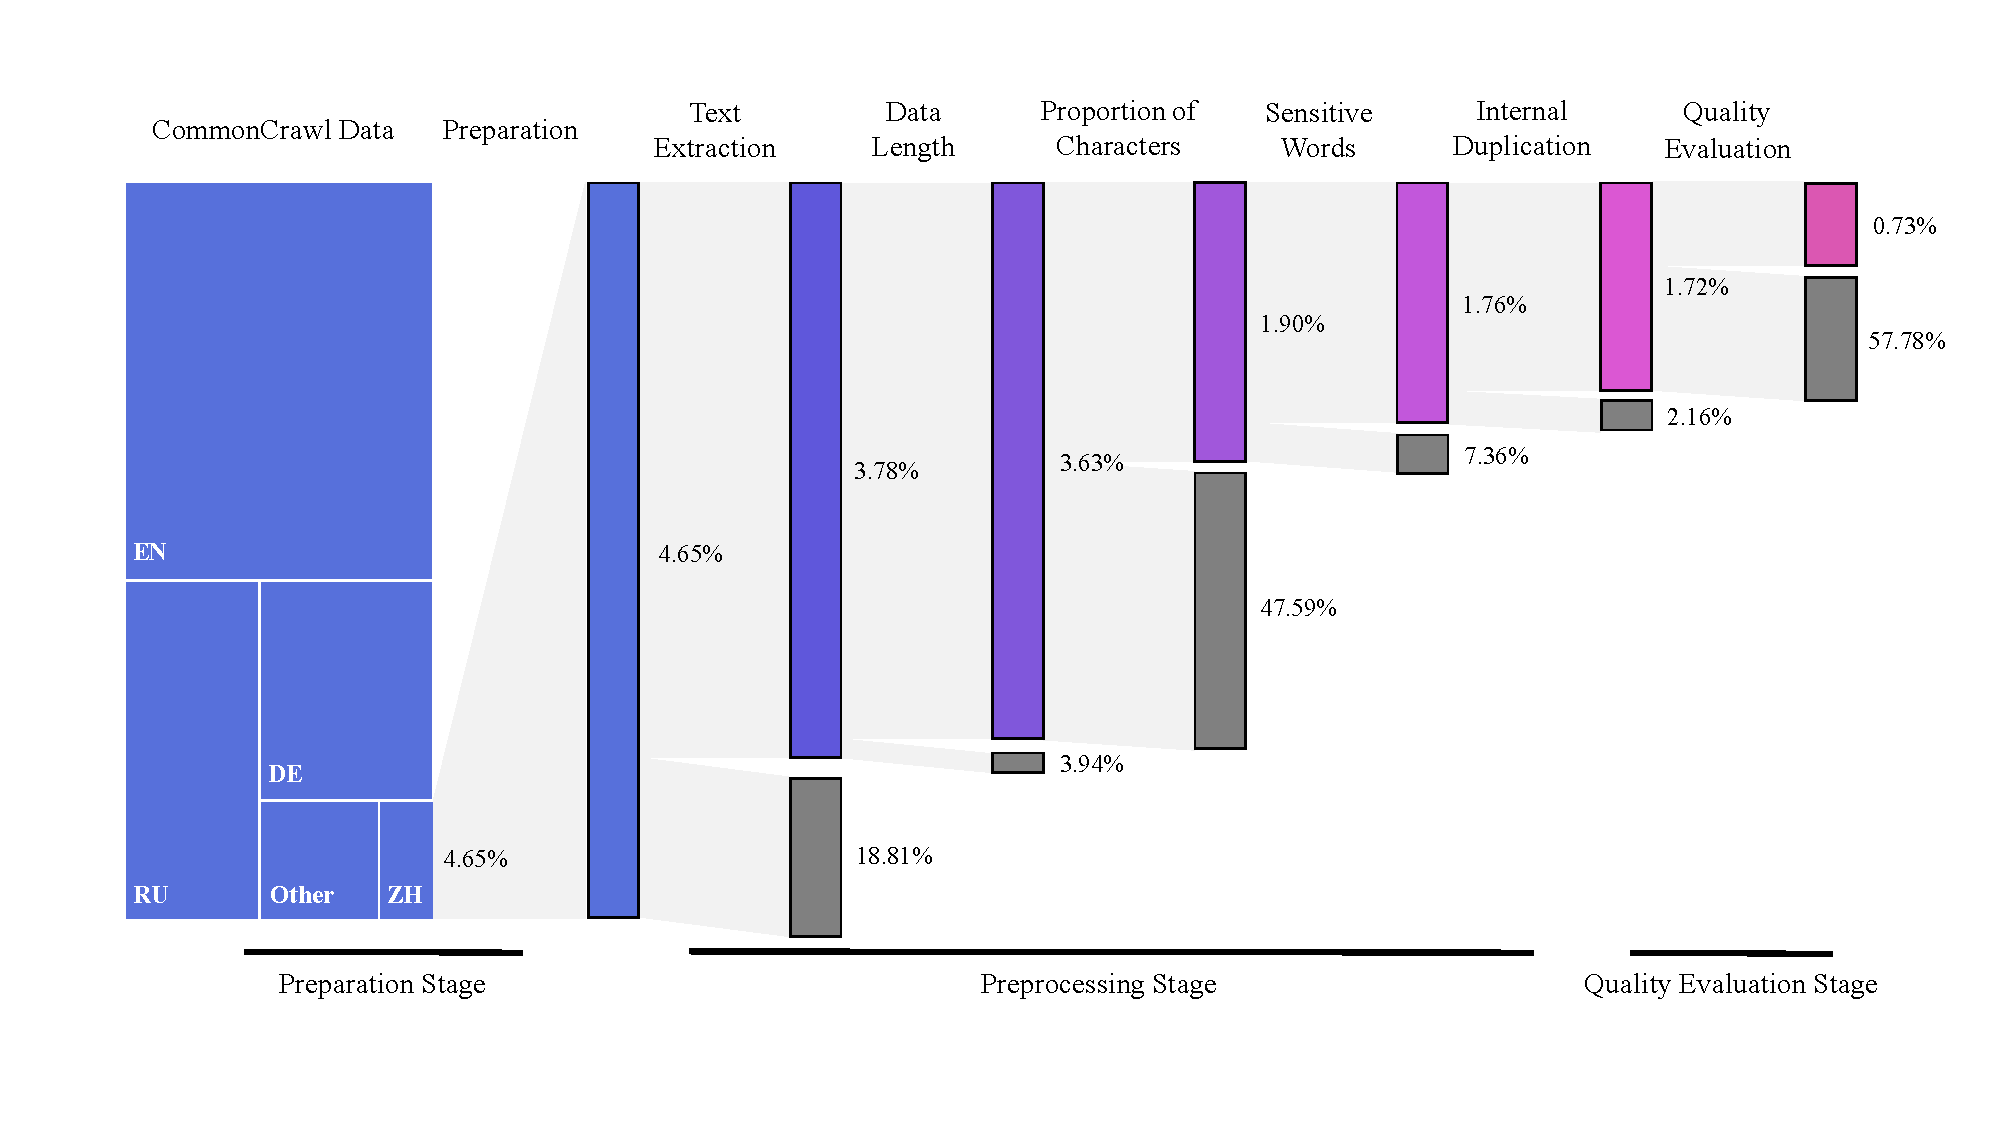
\includegraphics[width=0.95\textwidth]{picture/Ratio.pdf}
  \caption{Removal rate for different stages. Grey represents the removal rate with respect to each previous step, while other colors represent the kept rate of all data.}
  \label{fig4removal-rate}
\end{figure}

% As illustrated in Table \ref{remain_size} and Figure \ref{fig4removal-rate}, over half of the data is excluded during the preparation phase. This is primarily attributed to the removal of certain key-values generated by CCNet that do not offer substantial significance for subsequent analyses. And we filter all entries containing Traditional Chinese to ensure data consistency and purity. Building on this, a variety of manually defined criteria are employed to further refine the dataset, targeting the elimination of texts that either possess limited informational value, contain sensitive or inappropriate content, exhibit a low percentage of Chinese characters, or display redundant characteristics. Considering the disparity in filtering numbers between manual rule-based methods and model evaluation, it's clear that relying solely on rules falls short in eliminating low-quality text. This accentuates the necessity for a advanced evaluation model.


\subsection{Data Quality Distribution}

To investigate the relationship between data quality and data quantity, in this section, we adopt different quality thresholds to select data from our ChineseWebText dataset. As shown in Table \ref{data quality distribution}, it presents the high-quality data size for different threshold values. In this table, the value of threshold represents the proportion of selected data in the overall dataset. Then, we hire three human evaluators to assess the quality of the selected data for each threshold. The evaluation criteria has been outlined in section 3.4. 


\begin{table*}[htb]
\centering
    %\small
     \caption{The data quality distribution with different quality threshold.}
    \label{data quality distribution}
    \begin{tabular}{cccccc}
    \toprule
    \multirow{2.5}{*}{\textbf{Threshold}} & \multirow{2.5}{*}{\textbf{High Quality Data Size}}&         \multicolumn{4}{c}{\textbf{Accuracy}}\\
    \cmidrule{3-6}
    & & \#1 &  \#2 & \#3 &{Average} \\
    \midrule 
    25\% & 376.90 GB & 92.80\% & 94.80\% & 94.90\% & 94.17\%  \\  
    35\% & 525.59 GB & 93.60\% & 93.60\% & 93.10\% & 93.43\% \\ 
    40\% & 599.82 GB & 90.30\% & 91.90\% & 89.50\% & 90.57\%  \\
    45\% & 672.68 GB & 84.60\% & 85.50\% & 85.59\% & 85.33\% \\
    \bottomrule
    \end{tabular}
   
\end{table*}



From Table \ref{data quality distribution},
we can observe that a lower threshold leads to higher data quality, but results in smaller data size. For example, when we keep top 25\% of our ChineseWebText, the quality can be higher than 94\%, but the remaining data only accounts for 376.9 GB. The threshold of 40\% seems to be a good choice, and it can balance the data scale and data quality. The data size can reaches about 600 GB and the average data quality with human evaluation can be higher than 90\%. Therefore, this threshold is selected to construct the cleaner subset which is released along with our ChineseWebText. Anyway, our ChineseWebText could facilitate the LLMs researchers to choose their own high-quality dataset with their desired threshold.

%we can see that when we reduce the value of threshold, the size of the data significantly decreases, and the average accuracy of manual evaluation improves.  When the value of threshold is set to 40\%, the data size reaches 599.82 GB, and the average accuracy exceeds 90\%. This value ensures both the quality and scale of the data, and is therefore selected as the threshold of our cleaner subset, which has been presented in section 4.1. Based on ChineseWebText dataset, LLM researchers could also choose their own high-quality dataset with a desired threshold. 


%the size of selected data significantly decreases as the value of threshold decreases.
%it can be observed that when the threshold is set at 40\%, the data size reaches 599GB, and the average accuracy in the manual evaluation exceeds 90\%. This dataset is the cleaner dataset presented in section 3.4.



%From the very beginning, the quality of data is our top concern, especially for the quality of data in cleaner subset received relatively high scores and considered as high quality by the evaluation models. We measure the quality of data by evaluation models (see Section \ref{quality_evaluation}) and obtained high-quality data subset through quality control (see Section \ref{quality_control}). The quality score threshold, which judging whether the data is high-quality or not, is an important factor. This threshold is related to both the cleaner subset data quality and the data scale. As mentioned in Section \ref{dataset_statistics_comparison}, We define the threshold as a percentage of the evaluation scores of all data, that is, we consider the data with evaluation scores in the top 40\% as cleaner data. In order to choose the most appropriate threshold, we set multiple thresholds to filter ChineseWebText data and conduct human evaluation. The process and standards for human evaluation are the same as in Section \ref{quality_control}. For each threshold, data selected by this threshold is randomly sampled three times with 1000 samples. Each 1000 sampled data is evaluated by human to get the proportion of high quality data in the sampled data,i.e.,accuracy. We calculate the size of data filtered by each threshold and the average human evaluation accuracy over three sampling, with results shown in Table \ref{data quality distribution}.  

%Primarily, as shown in the table \ref{data quality distribution}, we select 40\% as the final threshold for cleaner data filtered from ChineseWebText, which ensures both a sufficiently large data scale (nearly 600GB) and higher data quality (average accuracy over 90\%). Secondly, the average accuracy corresponding to different thresholds reflect the powerful evaluation capabilities of our evaluation models. As the threshold changes from 45\% to 25\%, the average accuracy rises from 85.33\% to 94.17\%. A smaller threshold selects the data that evaluation model considered to be of higher quality, and the increase in average accuracy proves that the data does indeed have higher quality.
%Finally, this experiment can provide valuable insights for researchers to determine the appropriate thresholds. They can freely select thresholds according to their research requirements to filter data.







\subsection{Data Length Distribution}

During the training procedure of LLMs, longer texts can provide more abundant knowledge and information, making it easier for the models to understand complex relationships in the text, and learn more knowledge. In this section, we will analyze the length distribution of the texts in our cleaner dataset. As shown in Figure  \ref{fig4length}, it illustrates the distribution of text lengths within our cleaner Chinese subset.  From this figure, we can observe that the majority of text lengths are mainly distributed within 1000 characters or less. Among them, the most significant proportion is observed within the length interval of 300 to 500 characters. Texts exceeding 1000 characters account for a relatively small portion, and there is a long tail of very long texts. After analysis, we found that the maximum text length in this dataset can reach 300,000 characters. However, they are considered to be outliers and excluded from this figure. The text length distribution in this figure could provide valuable insights into the structure and characteristics of our cleaner subset, thereby help researchers in understanding the composition of the processed dataset and facilitating the utilization of the dataset.


%The length of data has a significant impact on pre-training. Therefore, we have analyzed the length distribution of the overall data, as shown in Figure \ref{fig4length}. Figure \ref{fig4length} presents the distribution of text lengths within the final filtered files. It is evident that the majority of the text falls within the range of $10^3$ characters or less. Among these, the most significant proportion is observed within the length interval of $3 \times 10^2$ to $5 \times 10^2$ characters. Texts exceeding $10^3$ characters constitute a relatively small portion, and their proportion decreases as the length increases. Notably, a few texts were observed to have lengths within the $4 \times 10^3$ to $3 \times 10^5$ characters. However, due to their minimal representation, they were not included in Figure \ref{fig4length}. The visual depiction of the text length distribution in Figure \ref{fig4length} serves to provide valuable insights into the structure and characteristics of the filtered documents, aiding researchers in understanding the composition of the processed data and facilitating the exploration of patterns and trends within the dataset.


\begin{figure}[htbp]
  \centering
  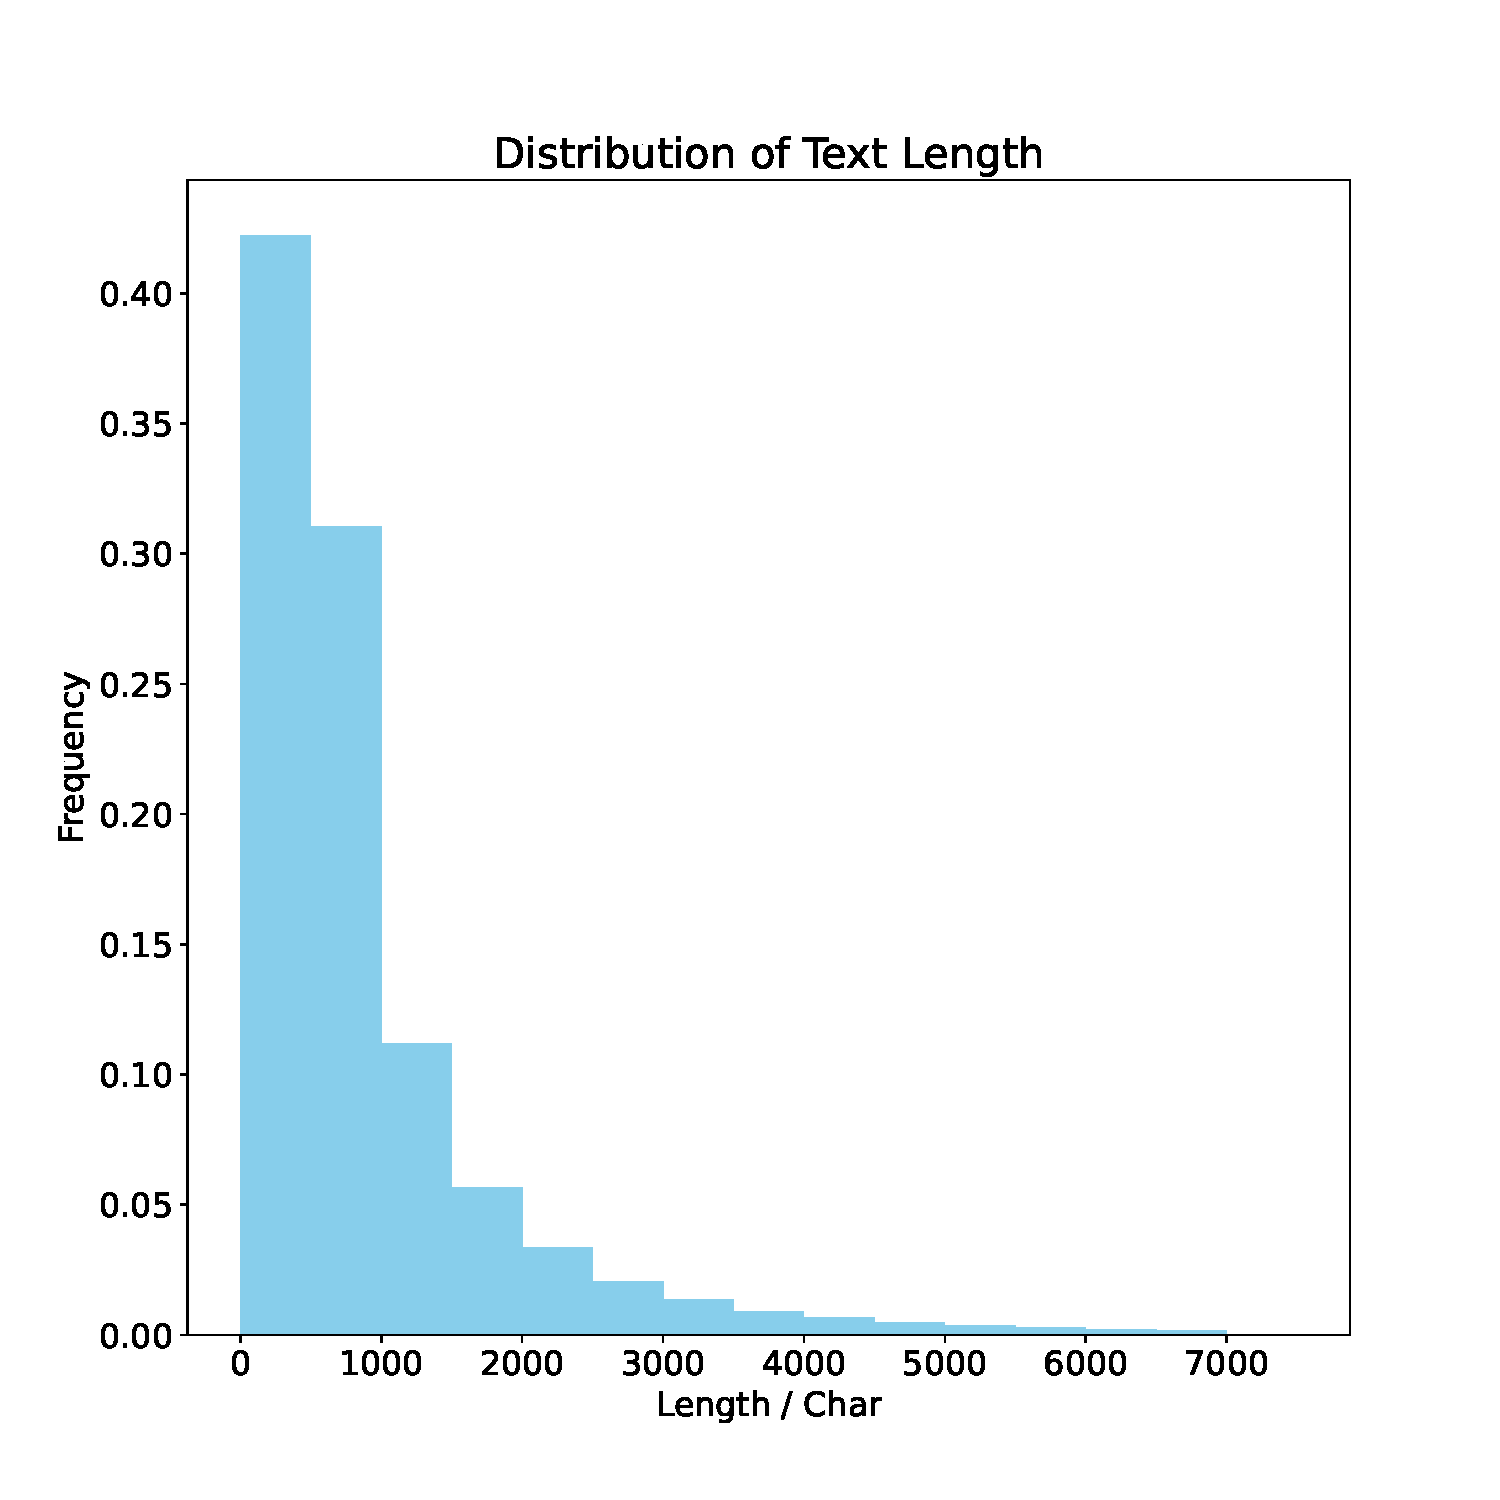
\includegraphics[width=0.6\textwidth]{picture/Length_analyze_bar.pdf}
  \caption{Length distribution of Data.}
  \label{fig4length}
\end{figure}





% \subsection{Evaluation Model Comparison}
% Here we first list two baseline quality evaluators: regression-based evaluator and perplexity-based evaluator.
% \subsubsection{Regression}
% We follow the work of \cite{gururangan_whose_2022} and employ a word frequency-based vectorization method in combination with logistic regression for text classification of the data. Logistic regression models the probability of data belonging to the positive class. We use logistic regression to calculate the evaluation probabilities for each sample. Then, we use these probabilities to determine whether each data point should be classified as positive or negative.
% \subsubsection{Perplexity}
% Perplexity measures the difficulty of a language model in predicting tokens and reflects the fluency of the data. Following the work of \cite{wenzek_ccnet_2020}, we utilize a language model to calculate the perplexity of data and classify it based on its perplexity score. We select data with lower perplexity values as positive samples.
% \subsubsection{Human Evaluation}
%  We randomly selected 300 samples and use Regression, Perplexity, FastText, BERTEval to assign scores. We evaluate the classification results by human evaluation. This leads to the subsequent question: how should high-quality text be defined? We believe that the following perspectives are important to measure the text quality.
 
 
% %   However, to the best of our knowledge, there are no metrics or evaluation methods in these perspectives for pre-training texts, except for toxicity. This constitutes a challenge in designing a web-crawling text quality filter.

% We calculated the proportion of positive examples classified by each model that accurately meets all four perspectives. A key point is that the objective of data classification is to improve the quality of data. And samples classified as positive will be used for further pre-training purposes. Therefore, we mainly focused on evaluating the precision, which indicates the proportion of truly positive samples. The results are presented in Table \ref{results}.The results indicate that both of our proposed methods, FastText, BERTEval, have shown impressive performance compared to Regression and Perplexity. Moreover, benefiting from the effect of data distillation, FastText's precision even surpassed BERTEval. 

% %\begin{table}[htbp]
% %	\caption{Classification Results }\label{results}
% % 	\centering
% % 	\begin{tabular}{lccc}
% % 		\toprule
% % 		Model      & Recall(\%) & F1(\%)  \\
% % 		\midrule\xrowht[()]{10pt}
% % 		Origin & 53 &  & \\ 
% % 		\xrowht[()]{10pt}
% % 		Regression & 49.57 & 72.96 & 59.03  \\
% % 		\xrowht[()]{10pt}
% % 		PPL &   &   &  \\
% % 		 \xrowht[()]{10pt}
% %         FastText&    &  & \\
% % 		\xrowht[()]{10pt}
% %         BERTEval & 73.79 & 47.80 & 58.02 \\	  
% % 		\bottomrule
% % 	\end{tabular}
% % \end{table}

% \begin{table}[htbp]
% 	\caption{Classification Results }\label{results}
% 	\centering
% 	\begin{tabular}{lccc}
% 		\toprule
% 		Model      & Precision(\%) & TP+FP & TP \\
% 		\midrule\xrowht[()]{10pt}
% 		Regression & 49.57 & 234 & 116 \\
% 		\xrowht[()]{10pt}
% 		Perplexity &  63.27 & 245 & 155 \\
% 		 \xrowht[()]{10pt}
% %         FastText&  \textbf{81.58} & 76 & 62 \\
% % 		\xrowht[()]{10pt}
%         BERTEval & 73.79 & 103 & \textbf{76}\\	  
% 		\bottomrule
% 	\end{tabular}
% \end{table}






\section{Conclusions and Future Work}
In order to extract large-scale and high-quality Chinese pre-training data from the web, we have proposed a new pipeline approach which filter the raw crawled web data with both handcrafted rules and well-designed quality evaluation model. The rules are employed to first extract the Chinese texts and remove duplicate documents, and then filter out the explicit noisy contents such as toxic texts and advertisements. The quality evaluation model is designed based on BERT and can assign each text with a quality score. With the proposed approach, we release the latest and largest Chinese dataset of 1.4 TB, each of which is associated with a quality score, facilitating the LLMs researchers to re-filter the data with desired quality thresholds. We further release a much cleaner subset of 600 GB Chinese data with the quality exceeding 90\% by human evaluation. We also release the complete tool-chain that processes the raw data into the clean texts.

In the future, we will continue to enlarge the Chinese dataset with newly incoming web data. Meanwhile, we are going to explore better algorithms and strategies for data filtering. For example, we can design quality evaluation models for each kind of data noise.

%a manual guided evaluation model. In this approach, we first adopt some manually crafted rules to filter the raw crawled web data. After that, a evaluation model is adopted to generate a quality score for each of the filtered data. Finally, the high-quality pre-training data can be filtered out with a appropriate threshold. Based on this approach, we process 3.9T raw web data and generate a 537 GB Chinese pre-training dataset. The results indicate that the accuracy of our final dataset could exceed 95\%, which could effectively meet the requirement of pre-training. Specifically, when publicly releasing our datasets, we not only provide the final high-quality dataset but also release the intermediate data with quality scores, allowing users to re-filter the data with new thresholds.
\bibliographystyle{unsrt}

\bibliography{references}  %%% Uncomment this line and comment out the ``thebibliography'' section below to use the external .bib file (using bibtex) .


%%% Uncomment this section and comment out the \bibliography{references} line above to use inline references.
% \begin{thebibliography}{1}

% 	\bibitem{kour2014real}
% 	George Kour and Raid Saabne.
% 	\newblock Real-time segmentation of on-line handwritten arabic script.
% 	\newblock In {\em Frontiers in Handwriting Recognition (ICFHR), 2014 14th
% 			International Conference on}, pages 417--422. IEEE, 2014.

% 	\bibitem{kour2014fast}
% 	George Kour and Raid Saabne.
% 	\newblock Fast classification of handwritten on-line arabic characters.
% 	\newblock In {\em Soft Computing and Pattern Recognition (SoCPaR), 2014 6th
% 			International Conference of}, pages 312--318. IEEE, 2014.

% 	\bibitem{hadash2018estimate}
% 	Guy Hadash, Einat Kermany, Boaz Carmeli, Ofer Lavi, George Kour, and Alon
% 	Jacovi.
% 	\newblock Estimate and replace: A novel approach to integrating deep neural
% 	networks with existing applications.
% 	\newblock {\em arXiv preprint arXiv:1804.09028}, 2018.

% \end{thebibliography}


\end{document}
